\chapter{Tool demonstration for load-following and safety analysis: 
Transatomic Power MSR}
In order to be competitive in the current domestic energy market, the 
\glspl{MSR} may need the flexibility to follow load. 
Load-following operation has the potential to increase the commercial 
competitiveness of nuclear power dramatically. Due to the increasing 
penetration of renewables into the electric grid, base-load operation carries 
the risk of correspondingly frequent negative electric energy pricing. Thus, 
responsiveness to the net electricity demand is essential to market relevance 
for new designs \cite{energy_information_administration_u.s._2016}.
This chapter presents a validation demonstration applying SaltProc v1.0 to 
simulate fuel salt depletion with online reprocessing during short-term 
transient to evaluate load-following capabilities of the \gls{TAP} \gls{MSR}.

\section{Technical aspects of load following with nuclear reactors}

The main physical effect that limits the possibilities of power variations in 
a conventional \gls{LWR} is fission product poisoning, especially iodine pit 
(the inability of the reactor to be started few hours after the reactor power 
decrease due to peak of $^{135}$Xe concentration in the core). The 
$^{135}$Xe is the most powerful known neutron absorber 
($\sigma_{a,^{135}Xe}=2.6\times10^6$ barns) with a half-life 
$\tau_{1/2}=9.17h$ and yield for $^{235}$U fission about 6.6\%. 
Figure~\ref{fig:xe-reaction-chain} shows the entire decay chain which 
characterizes $^{135}$Xe gain and loss channels. The vast 
majority of $^{135}$Xe (6.4\%) is produced from $^{135}$I decay 
($\tau_{1/2}=6.6h$). About half of $^{135}$I is produced directly from fission 
and half from $^{135}$Te decay ($\tau_{1/2}=19s$) 
\cite{nuclear_power_production_2020}.
\begin{figure}[hbp!] % replace 't' with 'b' to 
	\centering
	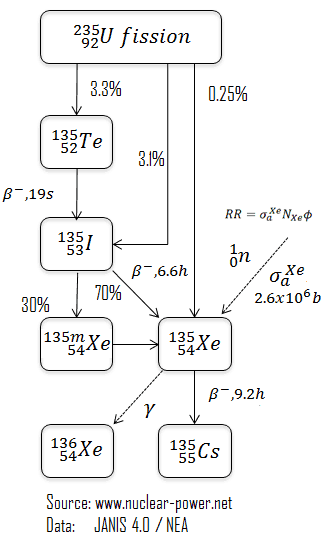
\includegraphics[width=0.4\textwidth]{ch5/xenon-135-reactions-decay.png}
	\caption{Mechanisms of $^{135}$Xe gain and loss in the reactor core 
		(figure reproduced from \cite{nuclear_power_production_2020}.}
	\label{fig:xe-reaction-chain}
\end{figure}

Under normal operating conditions, $^{135}$Xe is being 
transmuted to $^{136}$Xe ('burned out') in the reactor core as it is produced, 
so while it harms the neutron economy, balancing the reactor controls can 
compensate for its effect. The burn out of $^{135}$Xe for an operating reactor 
can be described as follows:
\begin{align}
& \isotope[135]{Xe}+\isotope[1]{n}\rightarrow \isotope[136]{Xe} \;(stable)
\end{align}
The difficulty comes when the reactor power is reduced, and there are fewer 
neutrons to burn out the $^{135}$Xe, so its concentration increases and 
further suppresses reactor power. In this case, the core takes some time to 
recover from the power reduction impact of $^{135}$Xe. This response to 
changing power levels, particularly from higher to lower power, 
dramatically slows the reactor's response to power demand
\cite{lokhov_load-following_2011}. 

In a liquid-fueled \gls{MSR}, gaseous fission products (e.g., xenon) can be 
dynamically removed from the fuel salt by the gas separation system (see 
Section~\ref{sec:gas-separ}). Thus, xenon gas, including problematic 
$^{135}$Xe, can be removed from the fuel salt outside of the reactor core to 
eliminate its negative impact on the core neutronics. If the vast majority of 
xenon can be removed, it is possible to alter the reactor power output in 
a wide range with very brief required recovery time. Overall, $^{135}$Xe 
removal during reactor operation will potentially allow precise and flexible 
dynamic control of reactor power level to follow power demands, typically 
referred to as `load following.'

This chapter presents modeling and simulation of load following transient 
operation of the \gls{TAP} \gls{MSR}. This study focuses on the 
$^{135}$Xe/$^{135}$I balance in the \gls{TAP} core and its effect on the 
reactor performance. In this chapter, I demonstrated the short-term ($<24$ 
hours) depletion simulation with the core power changing in the [0,100\%] 
range for xenon removal efficiency ($\epsilon_{Xe}$) varied between 0 and 
0.915 (see Table~\ref{tab:gas_removal_efficiency}). 

This chapter also demonstrates analysis of the reactor load-following 
capability for various moderator configurations and fuel salt compositions to 
bound desired efficiency of the gas removal system to ensure load-following 
operation. 

\section{TAP MSR load following analysis}
All of the analysis herein used SaltProc v1.0 with the full-core 3-D model of 
the \gls{TAP} \gls{MSR} developed using Serpent 2 (see 
Section~\ref{sec:tap_model}). The multi-component, online reprocessing system 
model with realistic noble gas removal efficiency described in 
Section~\ref{sec:tap-online-model} is used to simulate fission product removal 
and fresh fuel injection during anticipated transient. To be able to simulate 
transients with time-dependent power generation, I added to SaltProc v1.0 
capability to perform fuel salt depletion with variable depletion time step 
and reactor power level\footnote{For simplicity, the reactor power level is 
adjusted by changing normalization factor in Serpent (\emph{set power P[W]}). 
This simplification assumes that spatial and energy distribution of the 
neutron flux remains constant and only the magnitude of the flux changes with 
time. That is, control rod movement and corresponding change in the flux 
spatial and energy distribution is not treated here.} during each depletion 
step. The depletion calculation in load following regime capture the effects 
of $^{135}$Xe poisoning and evaluate the benefit of using an online gas 
removal system in the \gls{TAP} concept.

\subsection{Power load curve selection approach}
Load and generation must be continuously balanced almost instantly  in an 
electric power system. This is a physical requirement that independent on the 
market structure. Regulation and load following (which provided by intra-hour 
real-time energy market) are the two services required to continuously 
maintain balance between power generation and power load. 
Figure~\ref*{fig:power-curve-ny} demonstrates the morning ramp-up decomposed 
into total load (green), smooth load-following ramp (blue), and regulation 
(red). The smooth load-following slowly rises from 3566 MW to 4035 MW over 3 
hours. Regulation compensates for high-frequency fluctuations in the load 
around the underlying trend within $\pm55$MW range. In the PJM region 
(Delaware, Illinois, Indiana, Kentucky, Maryland, Michigan, New Jersey, North 
Carolina, Ohio, Pennsylvania, Tennessee, Virginia, West Virginia, and the 
District of Columbia), New York, and New England, the 5-min ramping capability 
of a generator is required for the regulation, while in Texas and California 
it is 15-min and 10-min, respectively \cite{kirby_method_2005}.
\begin{figure}[htp!] % replace 't' with 'b' to 
	\centering
	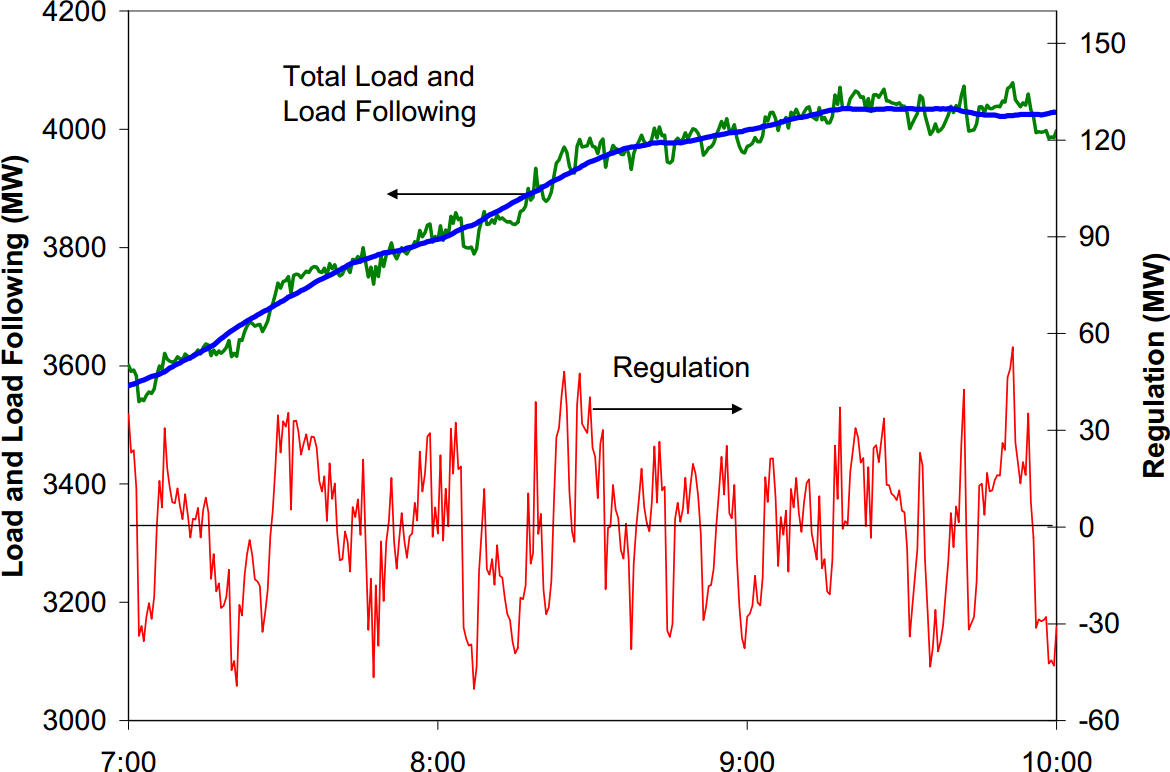
\includegraphics[width=0.85\textwidth]{ch5/power-curve-ny-morning.png}
	\caption{Regulation (red) compensates for minute-to-minute fluctuations in 
	system total load (green), load following (blue) compensates for the 
	inter- and 
	intra-hour ramps (figure reproduced from \cite{kirby_method_2005}).}
	\label{fig:power-curve-ny}
\end{figure}

In general, the regulation is the use of online generation or storage that is 
equipped with automatic generation control and is able to change output 
quickly (a few MW/min ramp rate) to compensate the minute-to-minute 
fluctuations in 
customer loads and correct for the unintentional fluctuation in power 
generation \cite{kirby_method_2005}. Typical natural gas peaking plant can 
ramp at or above 10\% of their capacity per minute \cite{huff_enabling_2018}. 
Elite combustion engine peakers (W\"{a}rtsil\"{a}) can ramp up from 10\% to 
100\% load (or down) in less than one minute \cite{wartsila_combustion_2020}.
Hydropower plants are also typically have very fast and accurate ramping 
capability which is suitable for regulation \cite{kirby_method_2005}.

Conventional nuclear power plants (Generation III/III+) can be used for 
load following (blue curve on Figure~\ref{fig:power-curve-ny}) but have 
limited maneuverability capabilities. For example, the German Konvoi reactors 
are designed for 15,000 cycles with daily power variations from 100\% to 60\% 
power level with ramp rate up to 2\%/min \cite{ludwig_load_2011} which is by 
order of magnitude slower than fossil-fueled plants. Ideally, we want to be 
able use nuclear power plants with \gls{MSR} to enable daily power variation 
with much more flexible range (from 100\% to 0\% and from 0\% to 100\%) and 
ramp rate up to 10\%/min to be competitive with thermal generators.

The physical effects that limit the possibilities of power variations in 
conventional \glspl{LWR} are \cite{lokhov_technical_2011}: (1) reactivity 
thermal feedback (change in the temperature of the primary coolant and fuel 
causes negative reactivity insertion which limits power regulation 
capabilities), (2) thermal strain and stress to fuel materials, (3) fuel 
burnup (low excess reactivity at the \gls{EOC}), and (4) \emph{$^{135}$Xe 
poisoning (iodine pit)}. Each of this physical effects is currently under 
thorough investigation of many researchers in several countries. However, 
\emph{the current chapter of the dissertation focuses only on $^{135}$Xe  
poisoning effect}. Other physical effects are not treated here.

Performing depletion calculation with SaltProc v1.0 to mimic load-following 
behavior shown on Figure~\ref{fig:power-curve-ny} would require very fine time 
step (e.g., 15-minute step). In order to simulate power change with desired 
rump rate (0.1 \gls{HFP}/min), less than 1-minute depletion time step is 
needed. 
Such fine resolution requires thousands depletion time steps to simulate 
12-hour transient involving unreasonable computational costs. 
Instead, this chapter presents simulations with 1-hour time step to 
investigate impact of gaseous fission products removal on the reactor's 
response to power demands. 

The most challenging power transient for conventional \glspl{LWR} from the 
viewpoint of xenon poisoning is well-defined in the literature: if after the 
$^{135}$Xe concentration reaches equilibrium (40-50 hours after startup with 
fresh fuel), the reactor power was decreased from 100\% to 0\% (e.g., the 
reactor is tripped), the $^{135}$Xe concentration and corresponding negative 
reactivity insertion would reach maximum in about 10-11 hours after shutdown 
\cite{lamarsh_introduction_1975, 
bell_nuclear_1970}. Preliminary study in the literature for the \gls{TAP} 
concept shown that the worst xenon impact on the core occurs in about 7.66 
hours after shutdown \cite{rykhlevskii_impact_2019}. Notably, the time after 
shutdown when $^{135}$Xe concentration reaches maximum is strongly depends on 
the reactor neutron energy spectrum.

Thus, to demonstrate SaltProc v1.0 capabilities for short-term transient with 
the reactor power change and to
investigate load-following capabilities of the \gls{TAP} reactor with focus on 
the xenon poisoning, I selected following worst-case power load profile:
\begin{enumerate}[label=(\alph*), noitemsep, topsep=0pt]
	\item Operate on 100\% of \gls{HFP} long enough to reach $^{135}$Xe 
	equilibrium;
	\item Instantaneous power drop from 100\% to 0\%;
	\item Shutdown for $t^{max}_X$ [hours] to reach the $^{135}$Xe 
	concentration extremum.
	\item Restart reactor instantly from 0\% to 100\% power level and operate 
	on 100\% for a few hours.
\end{enumerate}
This postulated worst-case transient can be considered as backing up solar 
power with 
nuclear on a high-solar-penetrated grid (e.g., in California).
Any other power load profile (i.e., blue load-following line shown in  
Figure~\ref{fig:power-curve-ny}) will demonstrate significantly milder xenon 
poisoning effect because the power demand change in the [0,100\%] range 
realistically is not instantaneous. That is, if the \gls{TAP} \gls{MSR} would 
be able to maintain criticality in the described stress test (e.g., 
$k_{eff}>1.0$ during all stages of the transient), than it is capable to 
follow realistic load curve.

To calculate time at which the $^{135}$Xe concentration will reach maximum, 
the following system of Ordinary Differential Equations (ODE) must be solved: 
\begin{align}
\frac{dI(t)}{dt} &= \gamma_I \Sigma_f\phi - \lambda_II \\
\frac{dX(t)}{dt} &= \lambda_II+\gamma_X\Sigma_f\phi - \lambda_XX - 
\sigma_{a,X}\phi X\\
\frac{dX(t)}{dt} &= 0
\intertext{where}
I, X &= \mbox{number density of $^{135}$I, $^{135}$Xe [cm$^{-3}$]} 
\nonumber\\
\gamma_I,\gamma_X &= \mbox{effective yield of $^{135}$I, $^{135}$Xe 
[fission$^{-1}$]} \nonumber\\
\lambda_I,\lambda_X &= \mbox{decay constant of $^{135}$I, $^{135}$Xe 
[s$^{-1}$]}\nonumber\\
\Sigma_f &= \mbox{macroscopic fission cross section of $^{235}$U [s$^{-1}$]} 
\nonumber\\
\sigma_{a,X} &= \mbox{microscopic absorption cross section of $^{135}$Xe 
[b]}\nonumber\\
\phi &= \mbox{neutron flux.}\nonumber
\end{align}
If the $^{135}$I and $^{135}$Xe concentrations at shutdown is $I_0$ and $X_0$, 
respectively, the time after shutdown when the $^{135}$Xe concentration peaks 
is given by:
\begin{align}\label{eq:time-xe-max}
t^{max}_X &= \frac{1}{\lambda_X-\lambda_I}
log(\frac{\lambda_X(\lambda_I[X_0+I_0]-\lambda_XX_0)}{\lambda_I^2 
I_0})
\end{align}

Since the $^{135}$I and $^{135}$Xe concentrations at shutdown in the \gls{TAP} 
core are expected to be different at the \gls{BOL} and \gls{EOL} due to 
significant spectral shift, $t^{max}_X$ is recalculated for each case to 
obtain the worst possible xenon poisoning effect. The ultimate goal of this 
effort is to evaluate impact of problematic fission products removal such as 
xenon on maximum negative reactivity insertion due to xenon poisoning and 
understand when it happens.

\subsection{Results and Analysis}
The \gls{TAP} full core depletion analysis was performed using SaltProc v1.0. 
I used 1-hour depletion time step during the transient to capture rapid 
changes in reactivity and isotopic composition. 
Figure~\ref{fig:lf-tap-keff-eol-eoc-no} demonstrated the effective 
multiplication factor evolution during postulated worst-case transient when 
the reactor is tripped for $11$ hours (typical time to reach maximum 
$^{135}$Xe concentration in conventional \glspl{LWR}) and then restarted. 
\emph{The gas removal system for 
that demonstration case was inactive to enhance xenon poisoning effect.}
At the beginning of the transient 
(initial conditions), the reactor operated for 8448 days ($\approx23$ years), 
all moderator rods are inserted in the core (see 1668 rods configuration in 
Figure~\ref{fig:tap-840-1668}). Negative effect of xenon poisoning is expected 
to be the greatest at the \gls{EOL} when the core has the most thermal neutron 
spectrum. 
Multiplication factor decreases by 64 $pcm$ during first two hours after 
shutdown ($^{135}$Xe concentration reached its maximum) and then increases by 
242 $pcm$ because $^{135}$Xe loss due to decay overcame its gain from 
$^{135}$I decay. The $k_{eff}$ increase accelerated after reactor power turned 
back to 100\% due to $^{135}$Xe burn out. 
Figure~\ref{fig:lf-tap-keff-eol-eoc-no} clearly indicates that the time after 
shutdown when the $^{135}$Xe reaches its extremum ($t^{max}_X$) for the 
\gls{TAP} reactor is significantly shorter than well-known xenon peak time for 
\glspl{LWR} (11 hours).

Using $^{135}$I and $^{135}$Xe concentrations at the beginning of the 
transient from long-term realistic analysis (see 
Section~\ref{sec:long-term-real}) and Equation~\ref{eq:time-xe-max}, I 
calculated the xenon peak time for the \gls{TAP} \gls{MSR} with all moderator 
rods inserted and fuel salt composition after 8448 days of operation 
$t^{max}_X=2.76h$. To estimate maximum negative reactivity insertion due to 
xenon poisoning, the transient simulation is repeated with the finer time 
resolution (15 minutes instead of 1 hour) and $t^{max}_X=2.75h$ to get maximum 
$^{135}$Xe concentration (Figure~\ref{fig:lf-tap-keff-eol-eoc-no-15}).
\begin{figure}[htp!] % replace 't' with 'b' to 
	\centering
	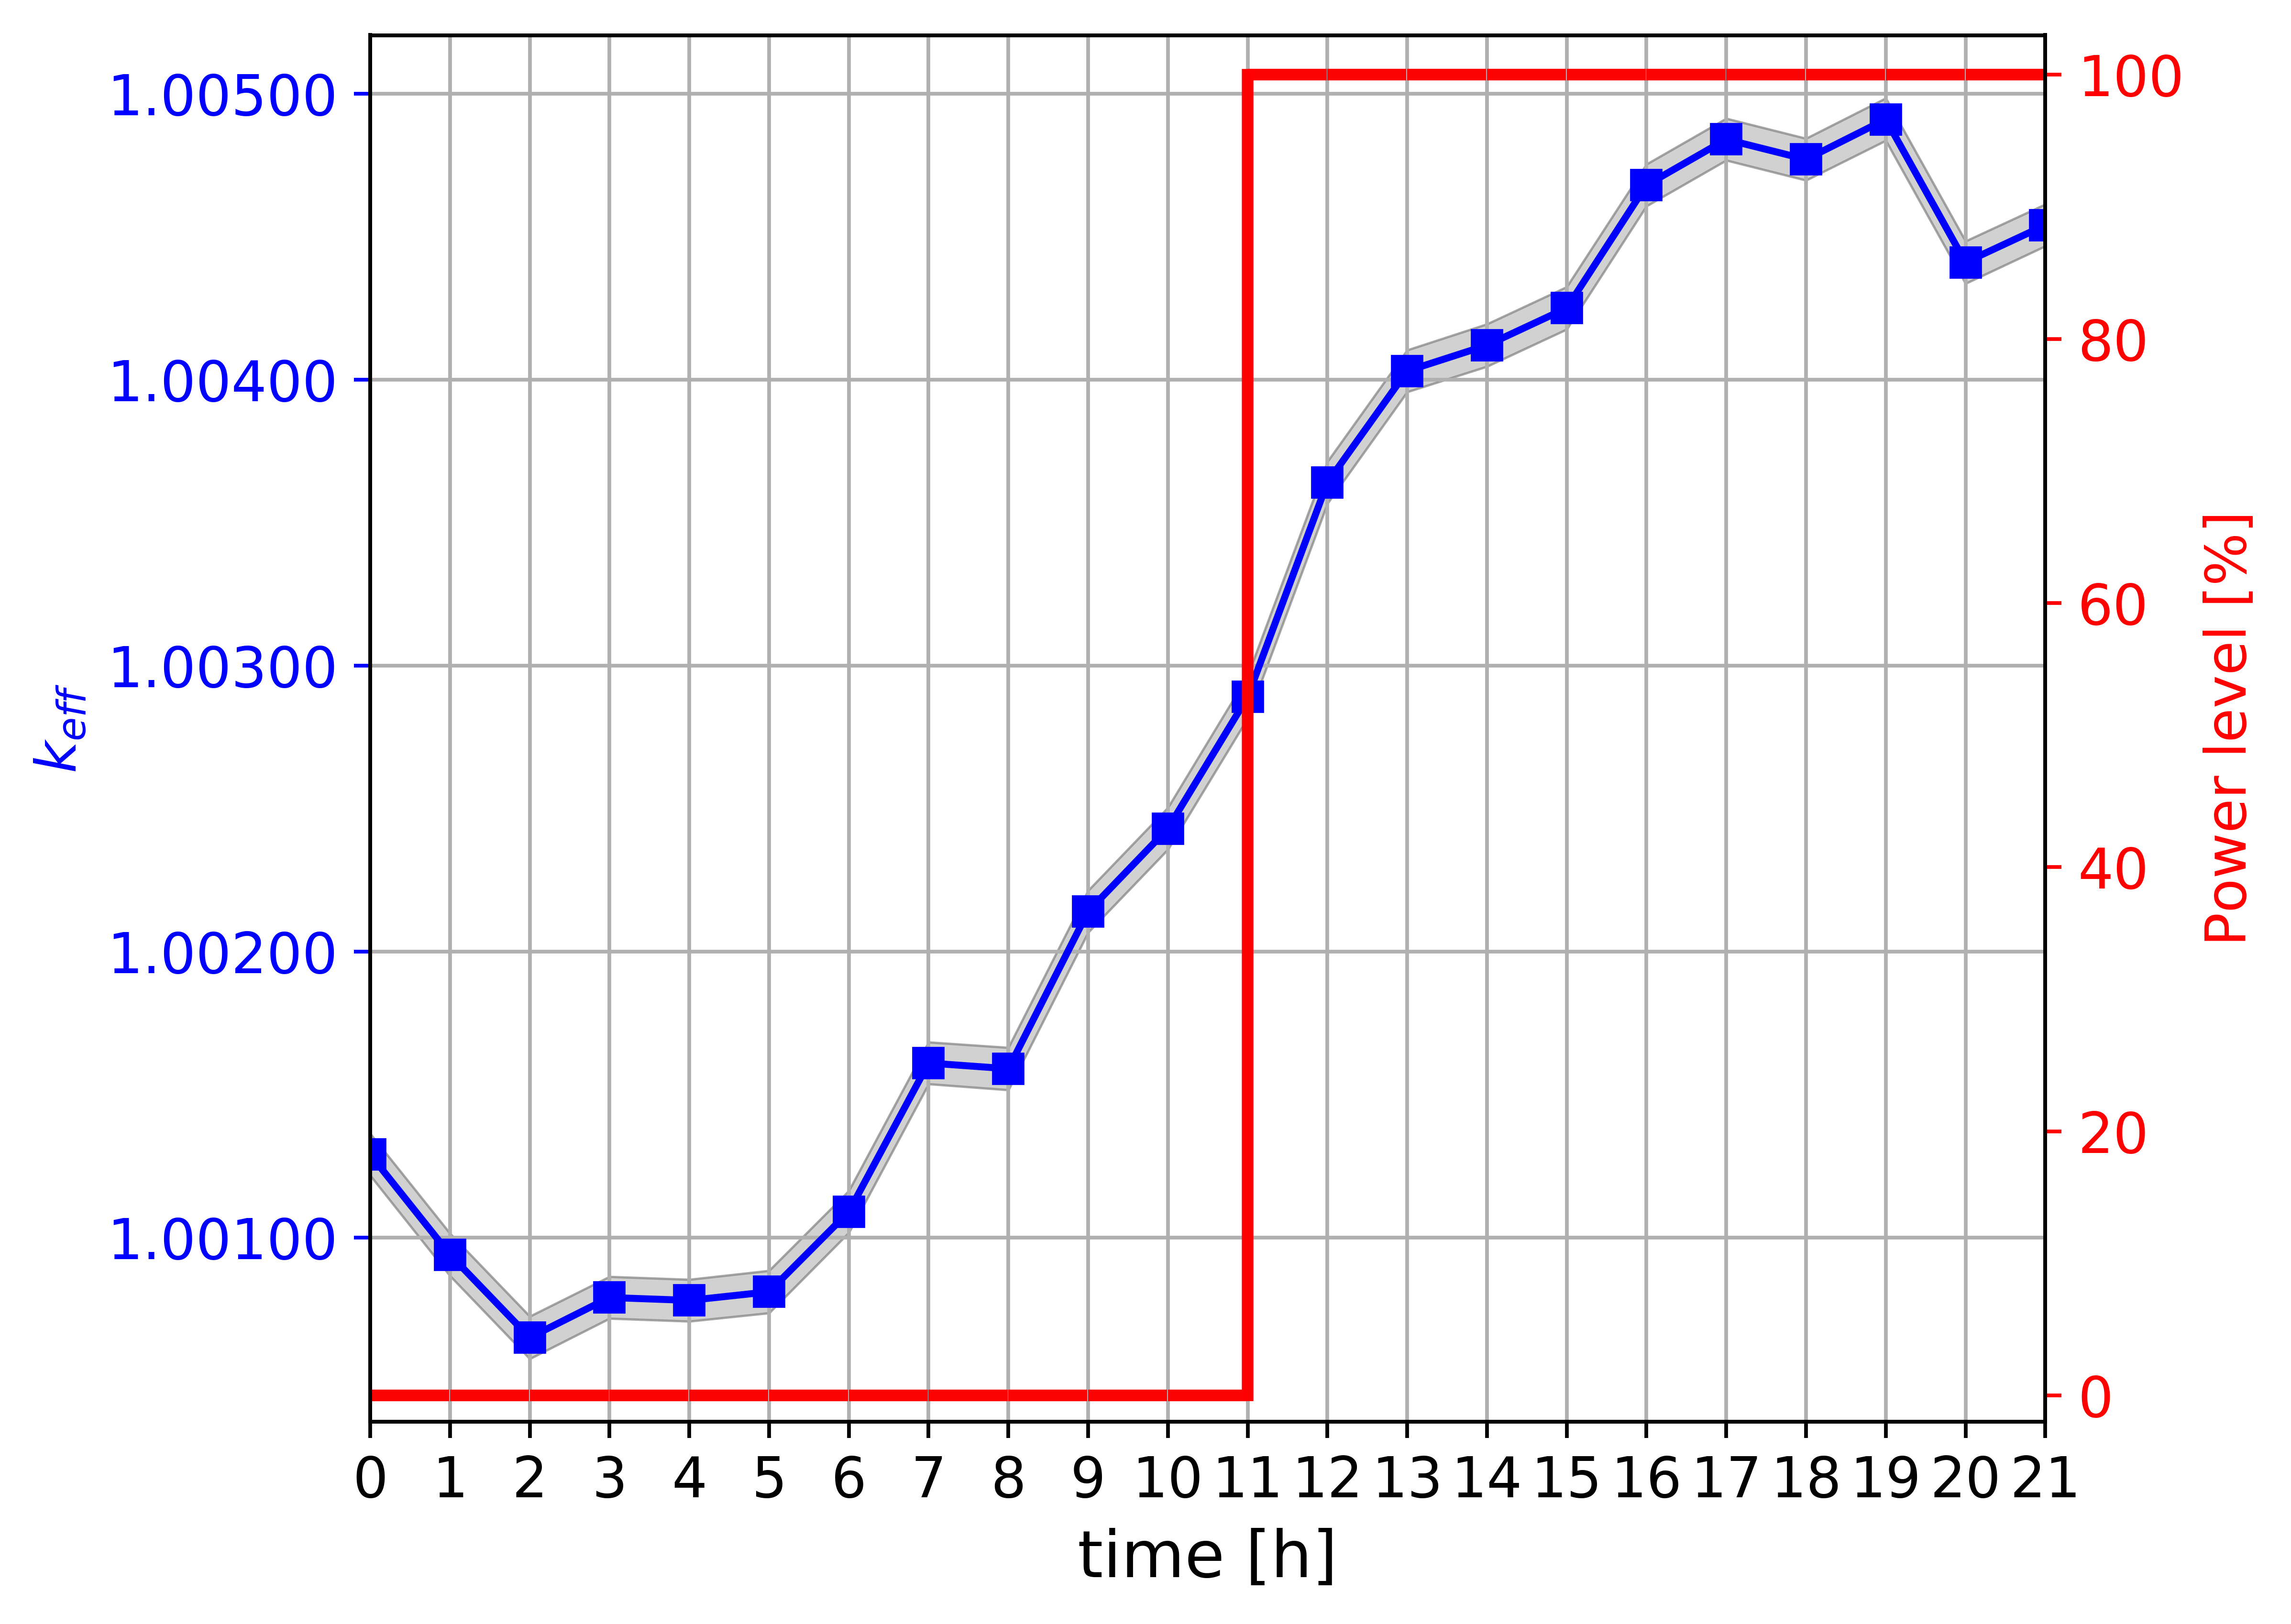
\includegraphics[width=0.9\textwidth]{ch5/keff_kl_1_eol_eoc.png}
	\caption{The effective multiplication factor dynamics for a 11-hour 
	shutdown (well-known xenon peak time for \glspl{LWR}) for the TAP reactor, 
	10 days before the \gls{EOL} (all moderator rods inserted), the gas 
	removal system is turned off. Uncertainty $\sigma\pm7$ $pcm$ is shaded.}
	\label{fig:lf-tap-keff-eol-eoc-no}
\end{figure}

Figure~\ref{fig:lf-tap-keff-eol-eoc-no-15} shows that the effective 
multiplication factor dropped by 70 $pcm$ during first 2.75 hours after 
shutdown as predicted by Equation~\ref{eq:time-xe-max}. After power ramp down 
from 0\% to 100\%, $k_{eff}$ returned to its initial value (1.00151) in 75 
minutes. The imbalance between $^{135}$I production and $^{135}$Xe burn out is 
the main reason of this positive reactivity boost. Notably, maximum negative 
reactivity insertion due to $^{135}$Xe buildup after shutdown in the 
\gls{PWR} is by order of magnitude greater than in the \gls{TAP} \gls{MSR}: 
$-1500$ $pcm$ \cite{rykhlevskii_impact_2019} and $-70$ $pcm$, respectively.
Thus, the \gls{TAP} core remains critical throughout worst-case power change 
even during the 10$^{th}$ day before the \gls{EOL} when operative excess 
reactivity is low ($151pcm>70pcm$). If the shutdown happens during last 9 days 
of the \gls{TAP} reactor operation with inactive gas removal system then the 
operator would not be able to restart it for awhile.
\begin{figure}[htp!] % replace 't' with 'b' to 
	\centering
	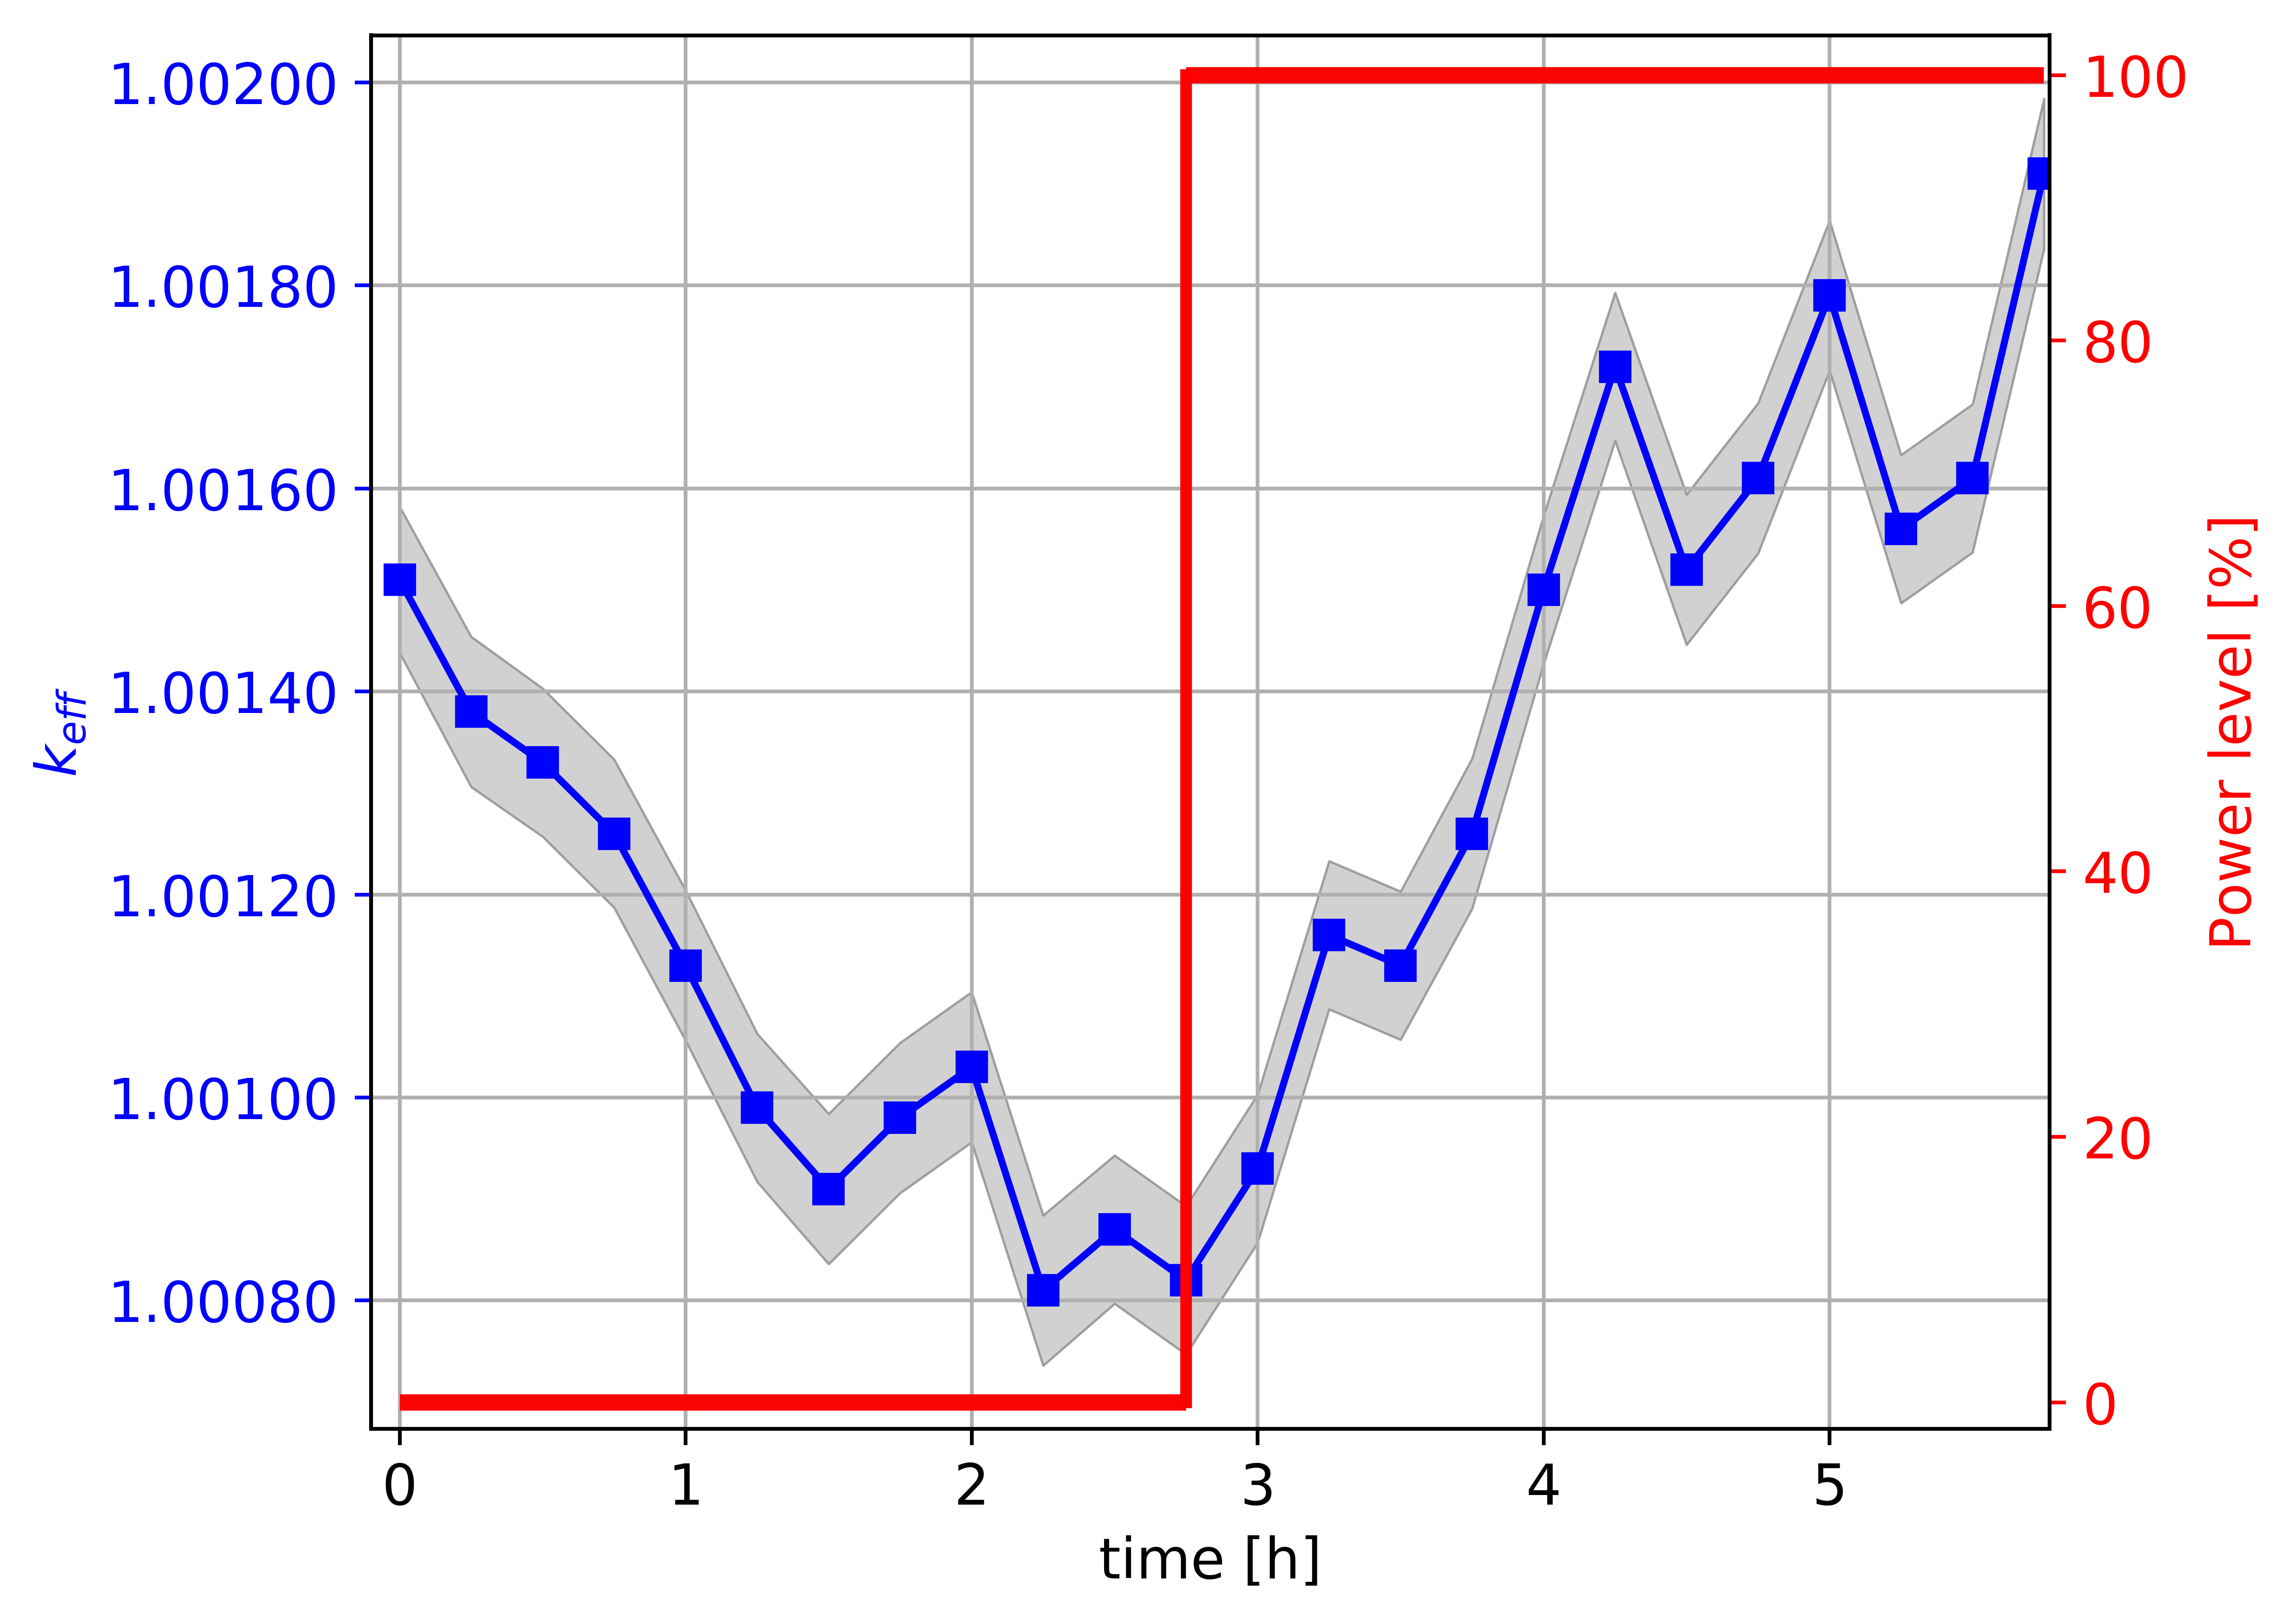
\includegraphics[width=0.9\textwidth]{ch5/keff_kl_1_eol_eoc_15min.png}
	\caption{The effective multiplication factor dynamics for the worst-case 
		load curve (2.75-hour shutdown) for the \gls{TAP} reactor, 10 days 
		before the \gls{EOL} (all moderator rods inserted), the gas removal 
		system is turned off. Uncertainty $\sigma\pm7$ $pcm$ is shaded.}
	\label{fig:lf-tap-keff-eol-eoc-no-15}
\end{figure}


The analysis of the fuel composition evolution provides clearer information 
about the $^{135}$Xe/$^{135}$I equilibrium and the core state. 
Figure~\ref{fig:lf-tap-xe-i-eol-eoc-no-15} shows the number density of 
isotopes influential to the \gls{TAP} core neutronics. The 
$^{135}$I/$^{135}$Xe number density ratio after reaching equilibrium is equal 
1.0. After shutdown, the $^{135}$I decays to $^{135}$Xe that is not burned up. 
The $^{135}$I decay caused xenon concentration 
peak by 4\% from equilibrium after 2.75 hours due to shorter $^{135}$I 
half-life ($\tau_{1/2}(^{135}I)=6.6$ $h$ vs. $\tau_{1/2}(^{135}Xe)=9.17$ 
$h$). Thus, $^{135}$Xe gain from $^{135}$I decay just slightly overcame 
$^{135}$Xe decay loss. In sum, the $^{135}$Xe peak is almost negligible (+4\%) 
even in worst-case load profile scenario due to much lower than for the 
\gls{PWR} $^{135}$I/$^{135}$Xe ratio at equilibrium: 1.0 and 2.3 
\cite{rykhlevskii_impact_2019} for the \gls{TAP} reactor and 
\gls{PWR}, respectively.
\begin{figure}[htp!] % replace 't' with 'b' to 
	\centering
	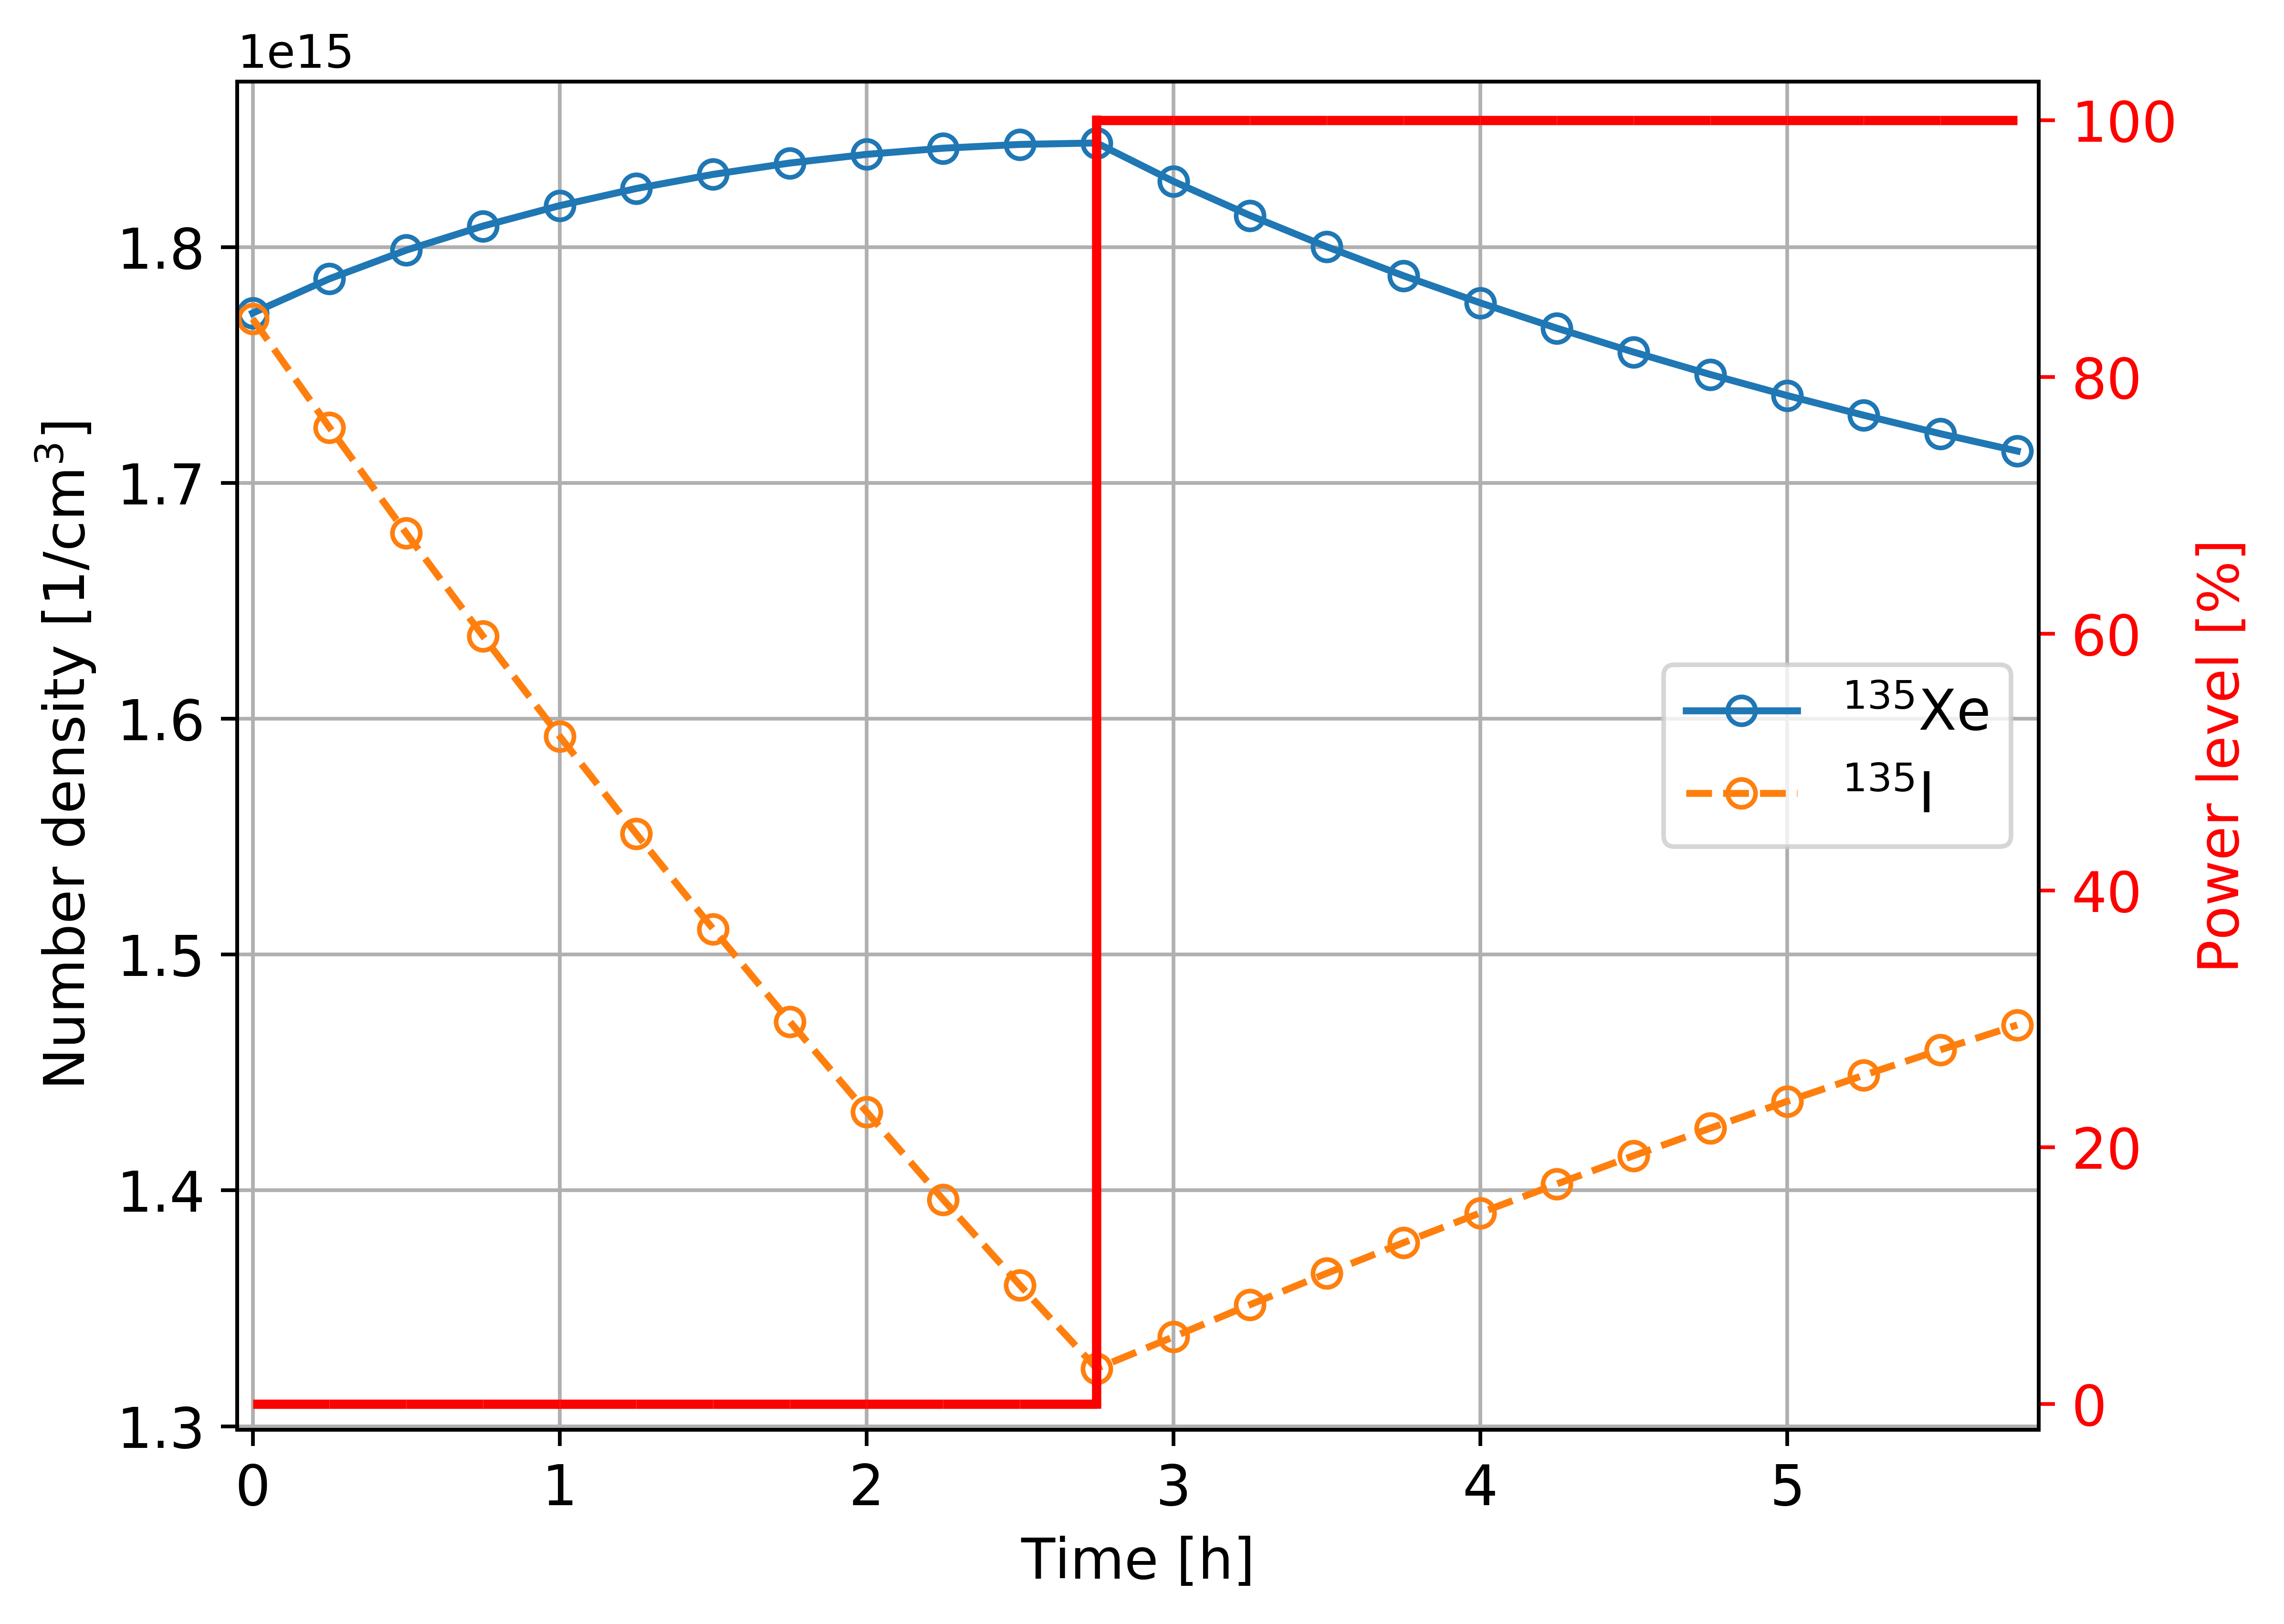
\includegraphics[width=0.9\textwidth]{ch5/xe_i_kl_1_eol_eoc_15min.png}
	\caption{Number density of $^{135}$Xe and its direct precursor $^{135}$I 
	for the worst-case load curve (2.75-hour shutdown) for the \gls{TAP} 
	reactor, 10 days before the \gls{EOL} (all moderator rods inserted), the 
	gas removal system is turned off.}
	\label{fig:lf-tap-xe-i-eol-eoc-no-15}
\end{figure}

Table~\ref{tab:lf-rho-change-eps-zero} summarizes results of above transient 
analysis for various moments during 23 years of the \gls{TAP} \gls{MSR} 
operation \emph{with inactive gas removal system}. I repeated the fuel 
composition and multiplication factor evolution analysis described earlier to 
evaluate impact of the reactor spectrum (geometry \#1 provided significantly 
harder spectrum than geometry \#15) and the fuel salt composition on the 
effect of xenon poisoning and, potentially, on the reactor's ability to 
follow load. 
The effect of xenon  poisoning worsens toward the \gls{EOL} because the 
$^{135}$Xe concentration peak is larger for the most thermal core 
configuration (all moderator rods inserted, largest possible moderator-to-fuel 
ratio). Right after last moderator configuration update, the xenon 
concentration peak is slightly larger than at the end of the cycle. The 
fissile $^{235}$U, $^{239}$Pu, and $^{241}$Pu concentration decreasing during 
last cycle due to burnup, while poisonous actinides (e.g., $^{238}$Pu, 
$^{240}$Pu, $^{242}$Pu, $^{236}$U) concentration keeps increasing which 
impacts the $^{135}$I/$^{135}$Xe number density ratio and, consequently, the 
$^{135}$Xe concentration peak value. Notably, such phenomena was not observed 
for the \gls{BOL} (geometry \#1, SVF=0.903) or \gls{MOL} (geometry \#8, 
SVF=0.766).
%%%%%%%%%%%%%%%%%%%%%%%%%%%%%%%%%%%%%%%%%%%%%%%%%%%%%%%%%%%%%%%%%%%%%%%%%%%%%%%
\begin{table}[htp!]
	\centering
	\caption{Effect of $^{135}$Xe poisoning after shutdown for the 
		\gls{TAP} reactor operation with inactive gas removal system		
		($\epsilon_{Xe}=0$). Stochastic uncertainty $\sigma_{\rho}=7$ 
		$pcm$.}
	\begin{tabularx}{\textwidth}{p{0.06\textwidth} p{0.03\textwidth} R R R R 
			R}
		\hline
		Geo\-metry &	SVF [-] & Time after moderator configuration update 
		[d] & Operative excess reactivity ($\rho_0$) [$pcm$] & Analytically 
		predicted $^{135}$Xe peak 
		time ($t^{max}_X$) [hr] & Maximum relative $^{135}$Xe concentration 
		change [\%] & Maximum reactivity change after shutdown ($\Delta\rho$) 
		[$pcm$] \\ \hline
		1 & 0.903 & startup & 3542 & 0.749 & +0.33 & -10  \\
		1 & 0.903 & 288     & 405  & 0.500 & +0.14 & -15  \\
		1 & 0.903 & 315     & 165  & 0.484 & +0.13 & -4   \\\hline
		8 & 0.766 & 3       & 3014 & 0.688 & +0.36 & -10  \\
		8 & 0.766 & 390     & 1529 & 0.722 & +0.39 & 0    \\
		8 & 0.766 & 777     & 204  & 0.751 & +0.42 & 0    \\\hline
		15& 0.536 & 3       & 2263 & 2.528 & +3.32 & -57  \\
		15& 0.536 & 153     & 1160 & 2.647 & +3.69 & -60  \\
		15& 0.536 & 297     & 129  & 2.758 & +4.07 & -70  \\
		\hline
	\end{tabularx}
	\label{tab:lf-rho-change-eps-zero}
\end{table}
%%%%%%%%%%%%%%%%%%%%%%%%%%%%%%%%%%%%%%%%%%%%%%%%%%%%%%%%%%%%%%%%%%%%%%%%%%%%%%%


Overall, the \gls{TAP} \gls{MSR} could be restarted after shutdown \emph{even 
without gas removal} 
in worst-case initial conditions: the most thermal moderator configuration, 
low operative excess reactivity at the end of the burn-up cycle, instantaneous 
power drop, and the $^{135}$Xe concentration at its extremum. To investigate 
effect of online fission gas removal on xenon poisoning effect, I repeated the 
worst-case load profile transient for different moments in time (e.g., 
\gls{BOL}, \gls{EOL}) and for the gas removal system operating with various 
xenon extraction efficiency ($\epsilon_{Xe}$). 

Figure~\ref{fig:lf-tap-rho-kl100-eol-eoc} shows reactivity change during the
\gls{TAP} reactor shutdown, 11 hours on 0\% power level, and following 
restart. In contrast with inactive gas removal system case, reactivity drops 
by 100 $pcm$ during first hour after the reactor shutdown. The $^{135}$Xe 
concentration is kept very low during long-term operation on 100\% because the 
gas removal system removed 91.5\% of xenon isotopes. At the same time, online 
reprocessing system did not remove $^{135}$I, hence, $^{135}$I/$^{135}$Xe 
concentration ratio is significantly greater than in no-removal case (11.0 vs. 
1.0). After shutdown, the $^{135}$I decays to $^{135}$Xe that 
is not burned up. According Equation~\ref{eq:time-xe-max}, the $^{135}$Xe 
concentration should reach local extremum in about 11 hours after shutdown, 
but this equation disregards the gas removal system operation. The depletion 
simulation using SaltProc v1.0 demonstrated that xenon concentration peaked in 
one hour after the shutdown and caused the reactivity drop by 100 $pcm$ (see 
Figure~\ref{fig:lf-tap-rho-kl100-eol-eoc}). The reactivity is quickly restored 
to its initial value during 3 hours after shutdown because the gas removal 
system removing 91.5\% of xenon every hour.

Table~\ref{tab:lf-rho-change-eps-1}  summarizes xenon poisoning analysis 
results for various moments during 23 years of \gls{TAP} \gls{MSR} operation 
\emph{with active gas removal system working with maximum efficiency}
($\epsilon_{Xe}=0.915$). Similar to the analysis with inactive gas removal 
system, maximum negative reactivity insertion due to xenon poisoning worsens 
toward the \gls{EOL} because the $^{135}$Xe concentration peak is greater for 
the core configuration with smaller SVF. Notably, the maximum $^{135}$Xe 
concentration rise is significantly greater for an excellent gas removal 
efficiency ($\epsilon_{Xe}=0.915$) than for the case with no gas removal 
($\epsilon_{Xe}=0$): +197\% and 4\%, respectively. Despite greater $^{135}$Xe 
concentration peak, negative change of reactivity after shutdown for the 
$\epsilon_{Xe}=0.915$ case is slightly deeper than for the 
$\epsilon_{Xe}=0$ case (-100 $pcm$ vs -70 $pcm$). The reason for this is the 
\gls{TAP} core neutron energy spectrum, which is harder than spectrum of 
conventional light-water thermal reactors. As we know, fast reactors are not 
affected by xenon poisoning because the absorption cross section of $^{135}$Xe 
in the fast spectrum is insignificantly larger than other fission products 
\cite{bell_nuclear_1970, 
svanstrom_load_2016-2}. The \gls{TAP} concept has intermediate spectrum which 
becomes more thermal towards the \gls{EOL}. Finally, the effect of xenon 
poisoning in \gls{TAP} \gls{MSR} is almost negligible and can be easily 
compensated by control rod movement, while in well-studied \gls{PWR} it is 
significantly greater ($-1500$ $pcm$) \cite{rykhlevskii_impact_2019}.
\begin{figure}[htp!] % replace 't' with 'b' to 
	\centering
	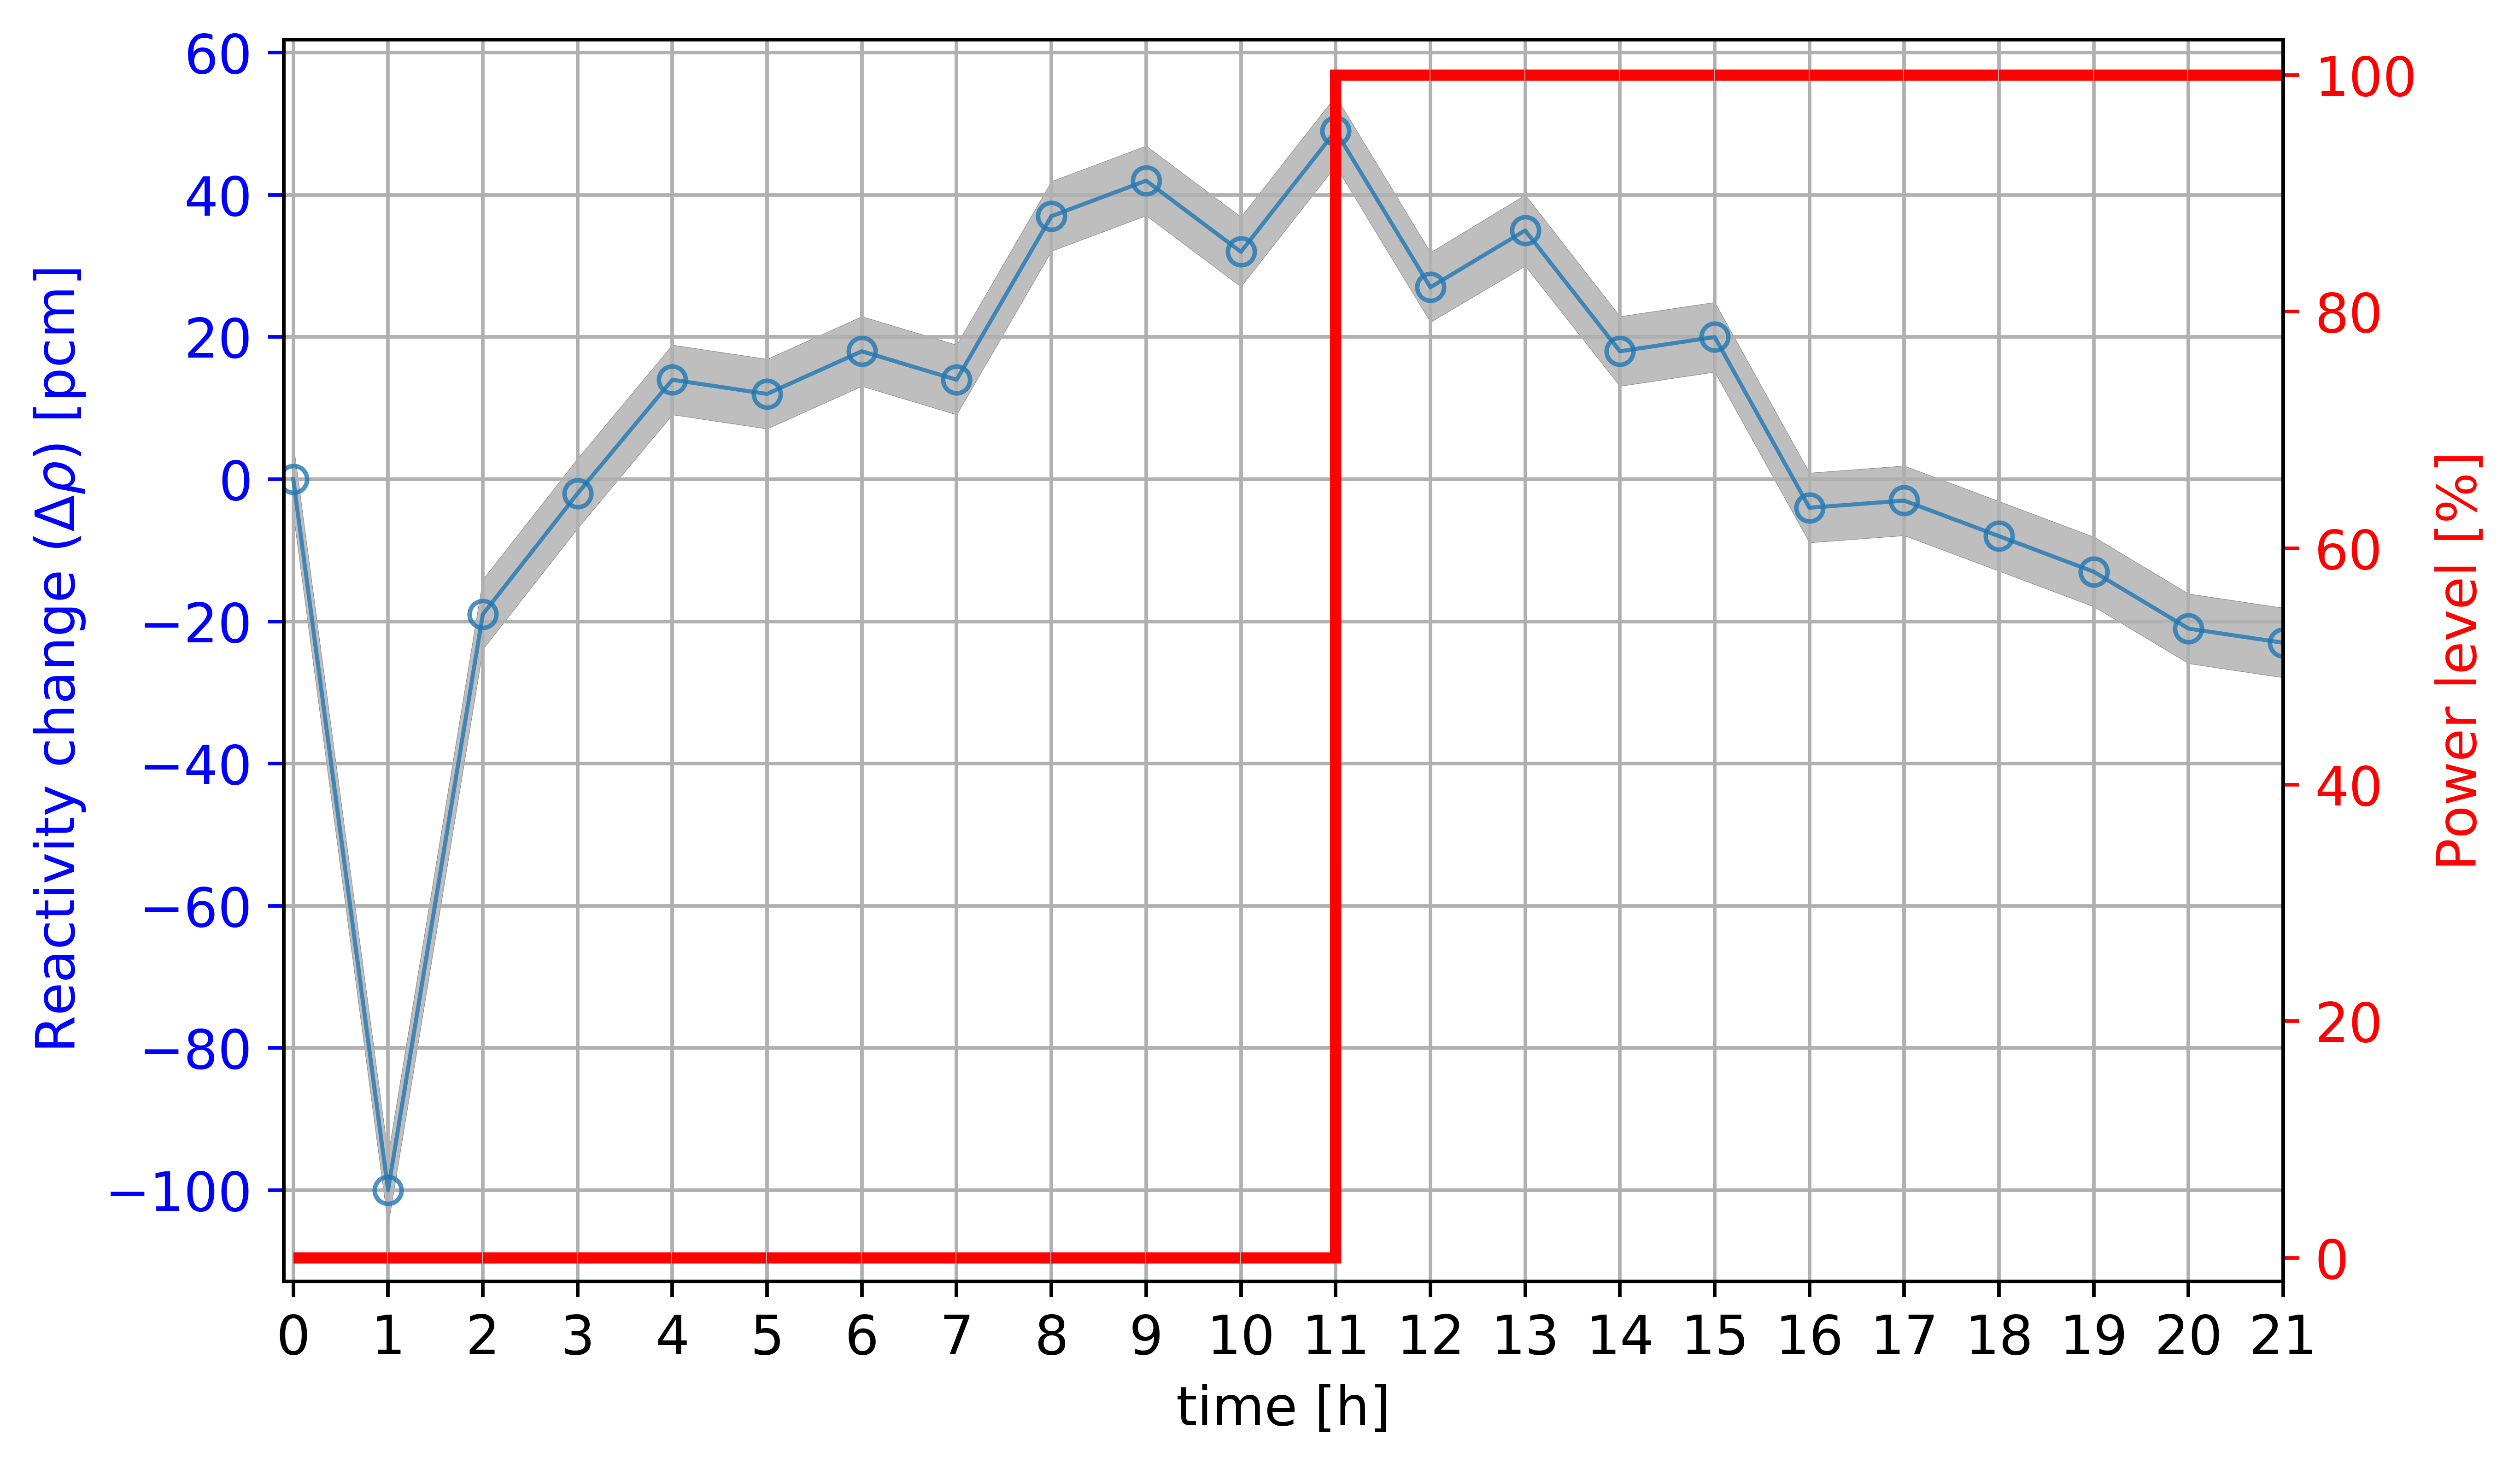
\includegraphics[width=0.97\textwidth]{ch5/rho_kl100_eol_eoc.png}
		\vspace{-5mm}
	\caption{Reactivity dynamics during a 11-hour shutdown for the 
		\gls{TAP} reactor, 10 days before the \gls{EOL} (all moderator rods 
		inserted), the gas removal system operates with efficiency 
		$\epsilon_{Xe}=0.915$. Uncertainty $\sigma\pm5$ $pcm$ is 
		shaded.}
	\label{fig:lf-tap-rho-kl100-eol-eoc}
\end{figure}
	\vspace{-5mm}
%%%%%%%%%%%%%%%%%%%%%%%%%%%%%%%%%%%%%%%%%%%%%%%%%%%%%%%%%%%%%%%%%%%%%%%%%%%%%%%
\begin{table}[hbp!]
	\centering
	\caption{Effect of $^{135}$Xe poisoning after shutdown for the 
		\gls{TAP} reactor operation with the high $^{135}$Xe removal 
		efficiency ($\epsilon_{Xe}=0.915$). Stochastic uncertainty 
		$\sigma_{\rho}=5$ $pcm$.}
	\begin{tabularx}{\textwidth}{p{0.06\textwidth} p{0.03\textwidth} R R R R 
			R}
		\hline
		Geo\-metry &	SVF [-] & Time after moderator configuration update 
		[d] & Operative excess reactivity ($\rho_0$) [$pcm$] & 
		$^{135}$I/$^{135}$Xe concentration ratio before shutdown
		[-] & Maximum relative $^{135}$Xe concentration 
		change [\%] & Maximum reactivity change after shutdown ($\Delta\rho$) 
		[$pcm$] \\ \hline
		1 & 0.903 & 9       & 3344 & 8.96  & +174 & -50  \\
    	1 & 0.903 & 171     & 1930 & 8.76  & +173 & -40  \\
		1 & 0.903 & 324     & 570  & 8.66  & +172 & -38  \\\hline
		8 & 0.766 & 3       & 3570 & 8.87  & +175 & -61  \\
		8 & 0.766 & 366     & 2150 & 8.90  & +174 & -40  \\
		8 & 0.766 & 762     & 762  & 8.93  & +175 & -33  \\\hline
		15& 0.536 & 9       & 3370 & 11.07 & +194 & -105  \\
		15& 0.536 & 90      & 2771 & 11.17 & +195 & -108  \\
		15& 0.536 & 303     & 1265 & 11.42 & +197 & -100  \\
		\hline
	\end{tabularx}
	\label{tab:lf-rho-change-eps-1}
\end{table}
%%%%%%%%%%%%%%%%%%%%%%%%%%%%%%%%%%%%%%%%%%%%%%%%%%%%%%%%%%%%%%%%%%%%%%%%%%%%%%%

To understand the difference between $^{135}$I/$^{135}$Xe gain and loss for 
the \gls{TAP} \gls{MSR} and \gls{PWR}, the neutron spectrum of both reactors 
must be analyzed. Figure~\ref{fig:tap-pwr-spectrum} 
demonstrates the neutron flux energy distribution normalized by unit lethargy 
for both reactors. The \gls{TAP} reactor spectrum at the \gls{BOL} (SVF=0.903) 
is much harder than for the \gls{PWR} due to lack of moderation in the 
\gls{TAP} core and its type (ZrH$_{1.66}$ instead of light water). The harder 
neutron spectrum leads to weaker $^{135}$Xe transmutation because capture 
cross section is declined rapidly with energy (see 
Figure~\ref{fig:tap-pwr-spectrum}, lower plot, solid red line, energy range 
from $10^{-7}$ to $10^{-4}$ MeV). As a result, the $^{135}$I/$^{135}$Xe number 
density ratio is 0.78 for the \gls{TAP} \gls{MSR} at the \gls{BOL} 
which is 3 times lower than that ratio for the \gls{PWR} with fresh fuel 
(2.3). Thus, the $^{135}$Xe gain from $^{135}$I decay cannot overcome 
$^{135}$Xe, and no xenon concentration peak is observed at the \gls{BOL} 
(Table~\ref{tab:lf-rho-change-eps-zero}, first three rows).
\begin{figure}[hbp!] % replace 't' with 'b' to 
	\centering
	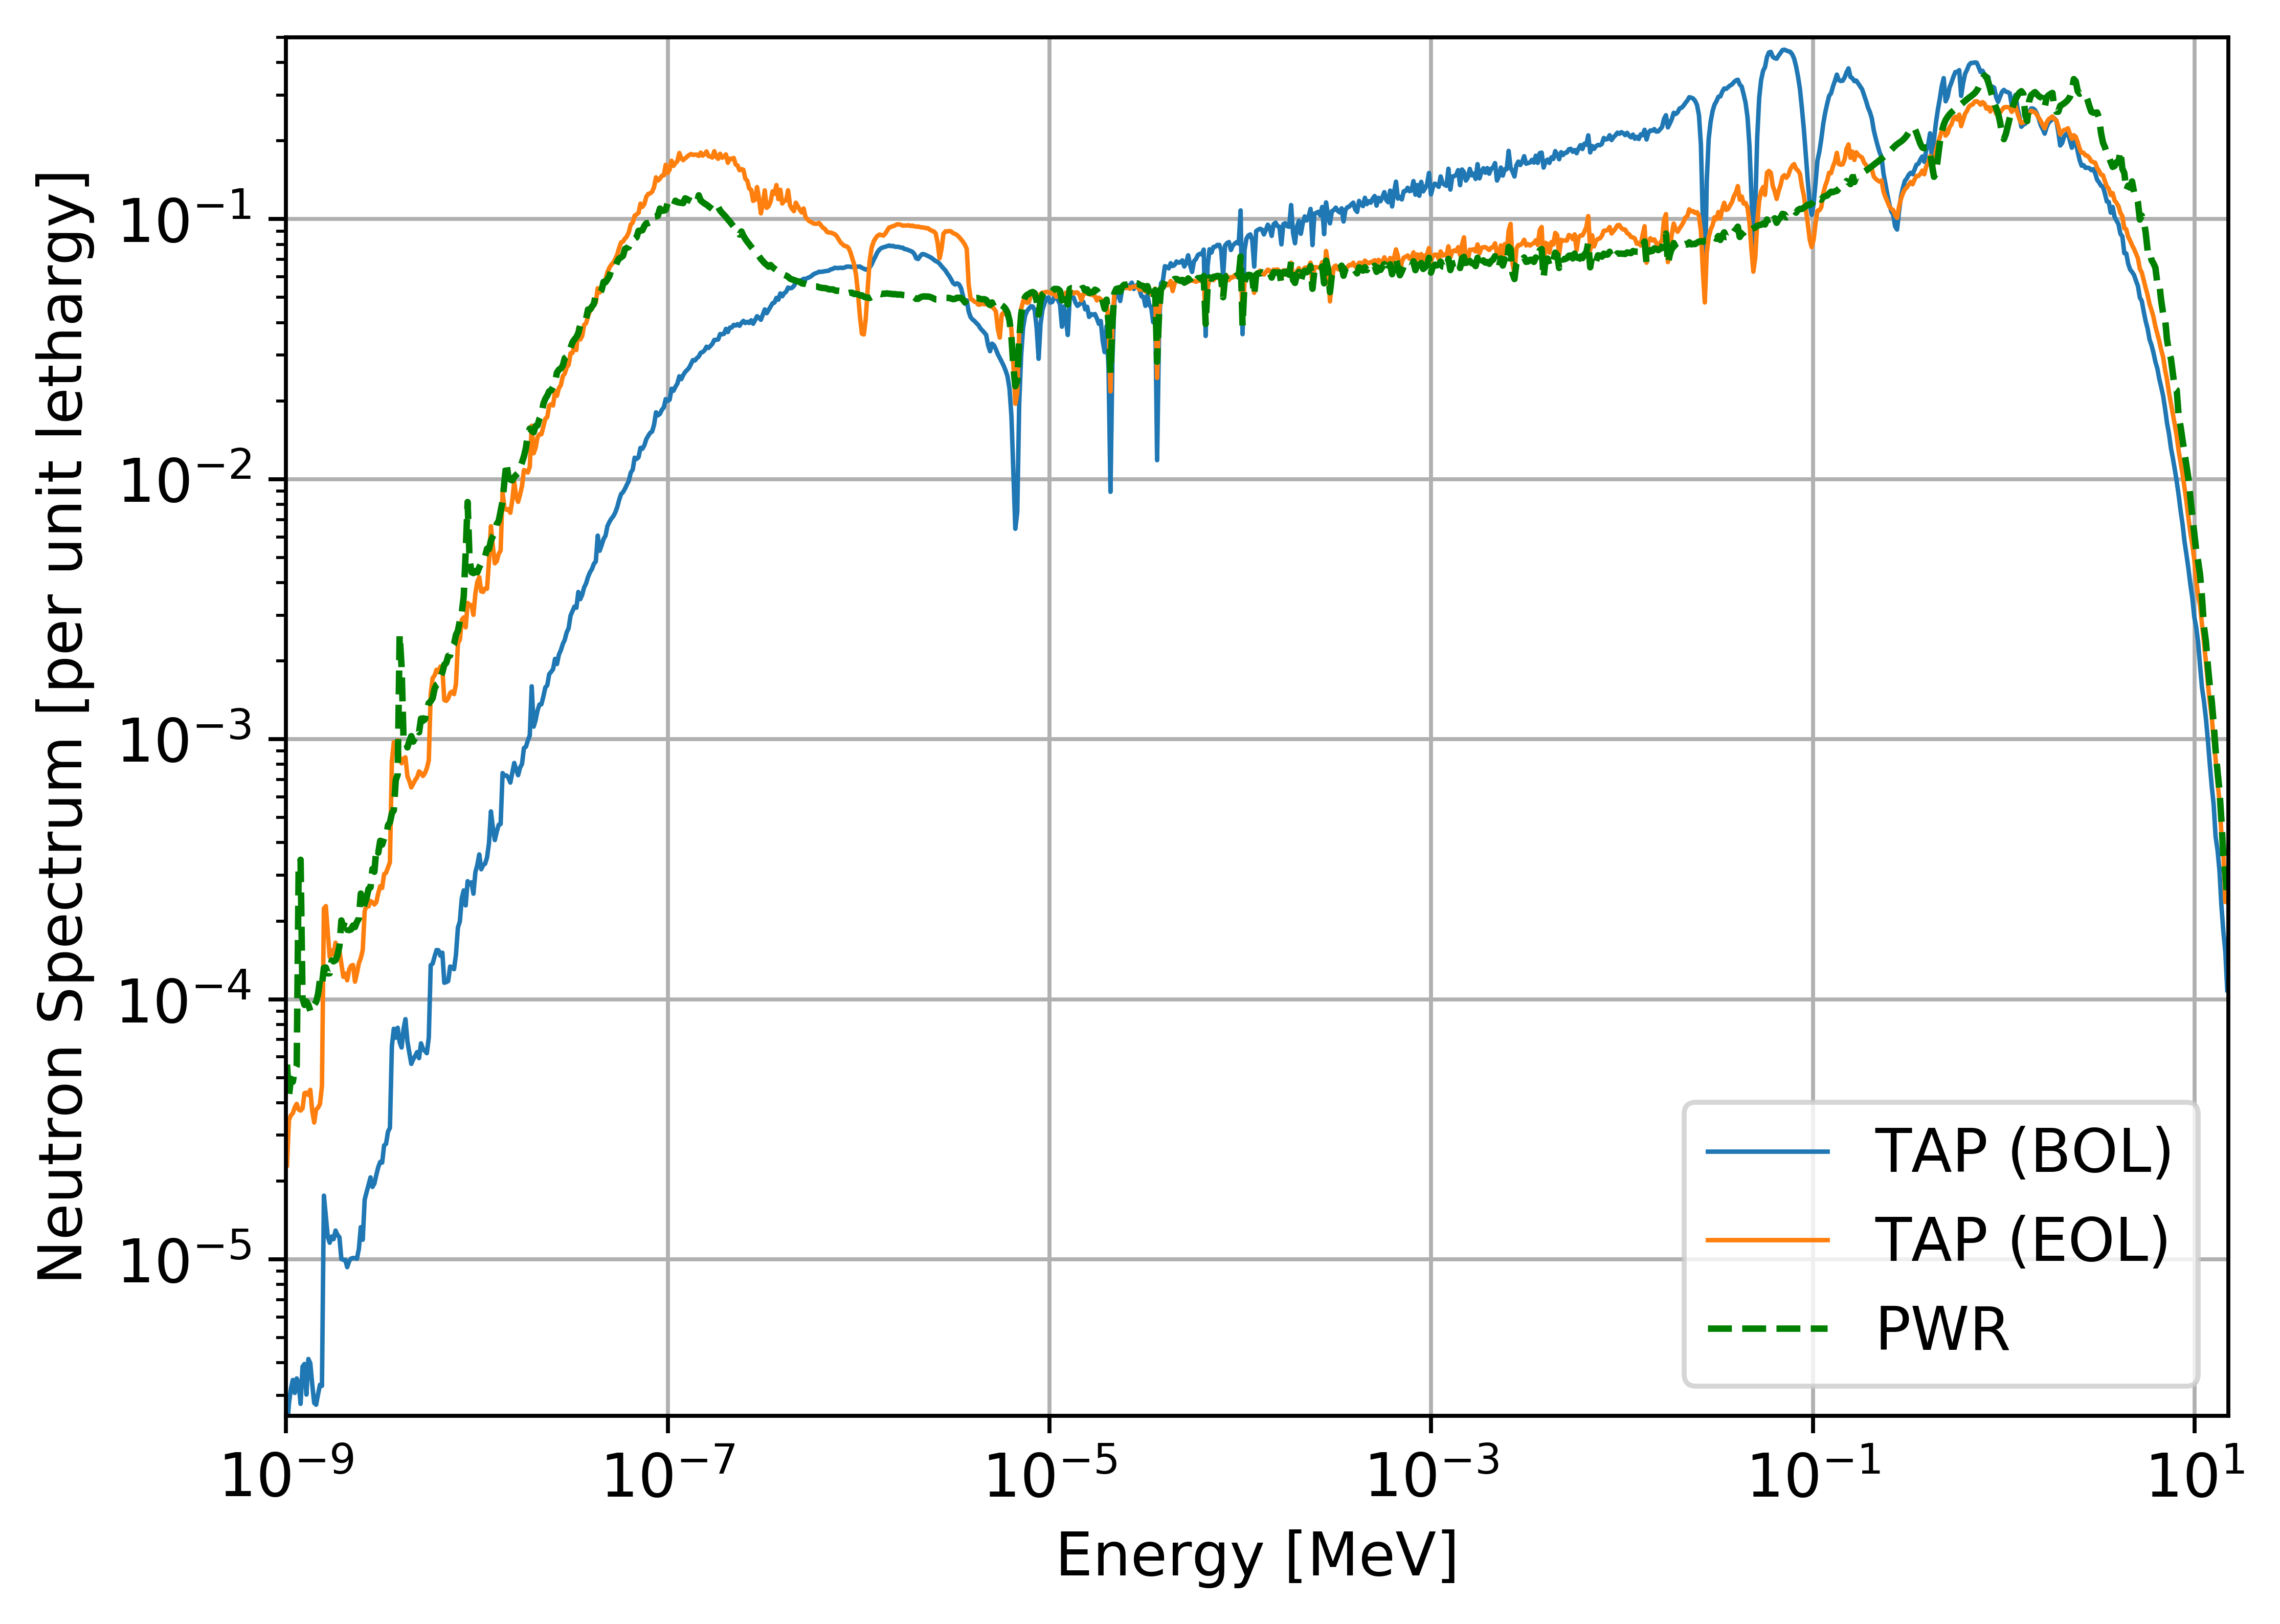
\includegraphics[width=\textwidth]{ch5/tap_vs_pwr_spectrum_2.png}\\
	\vspace{-19mm}
	\hspace{+0.05mm}
	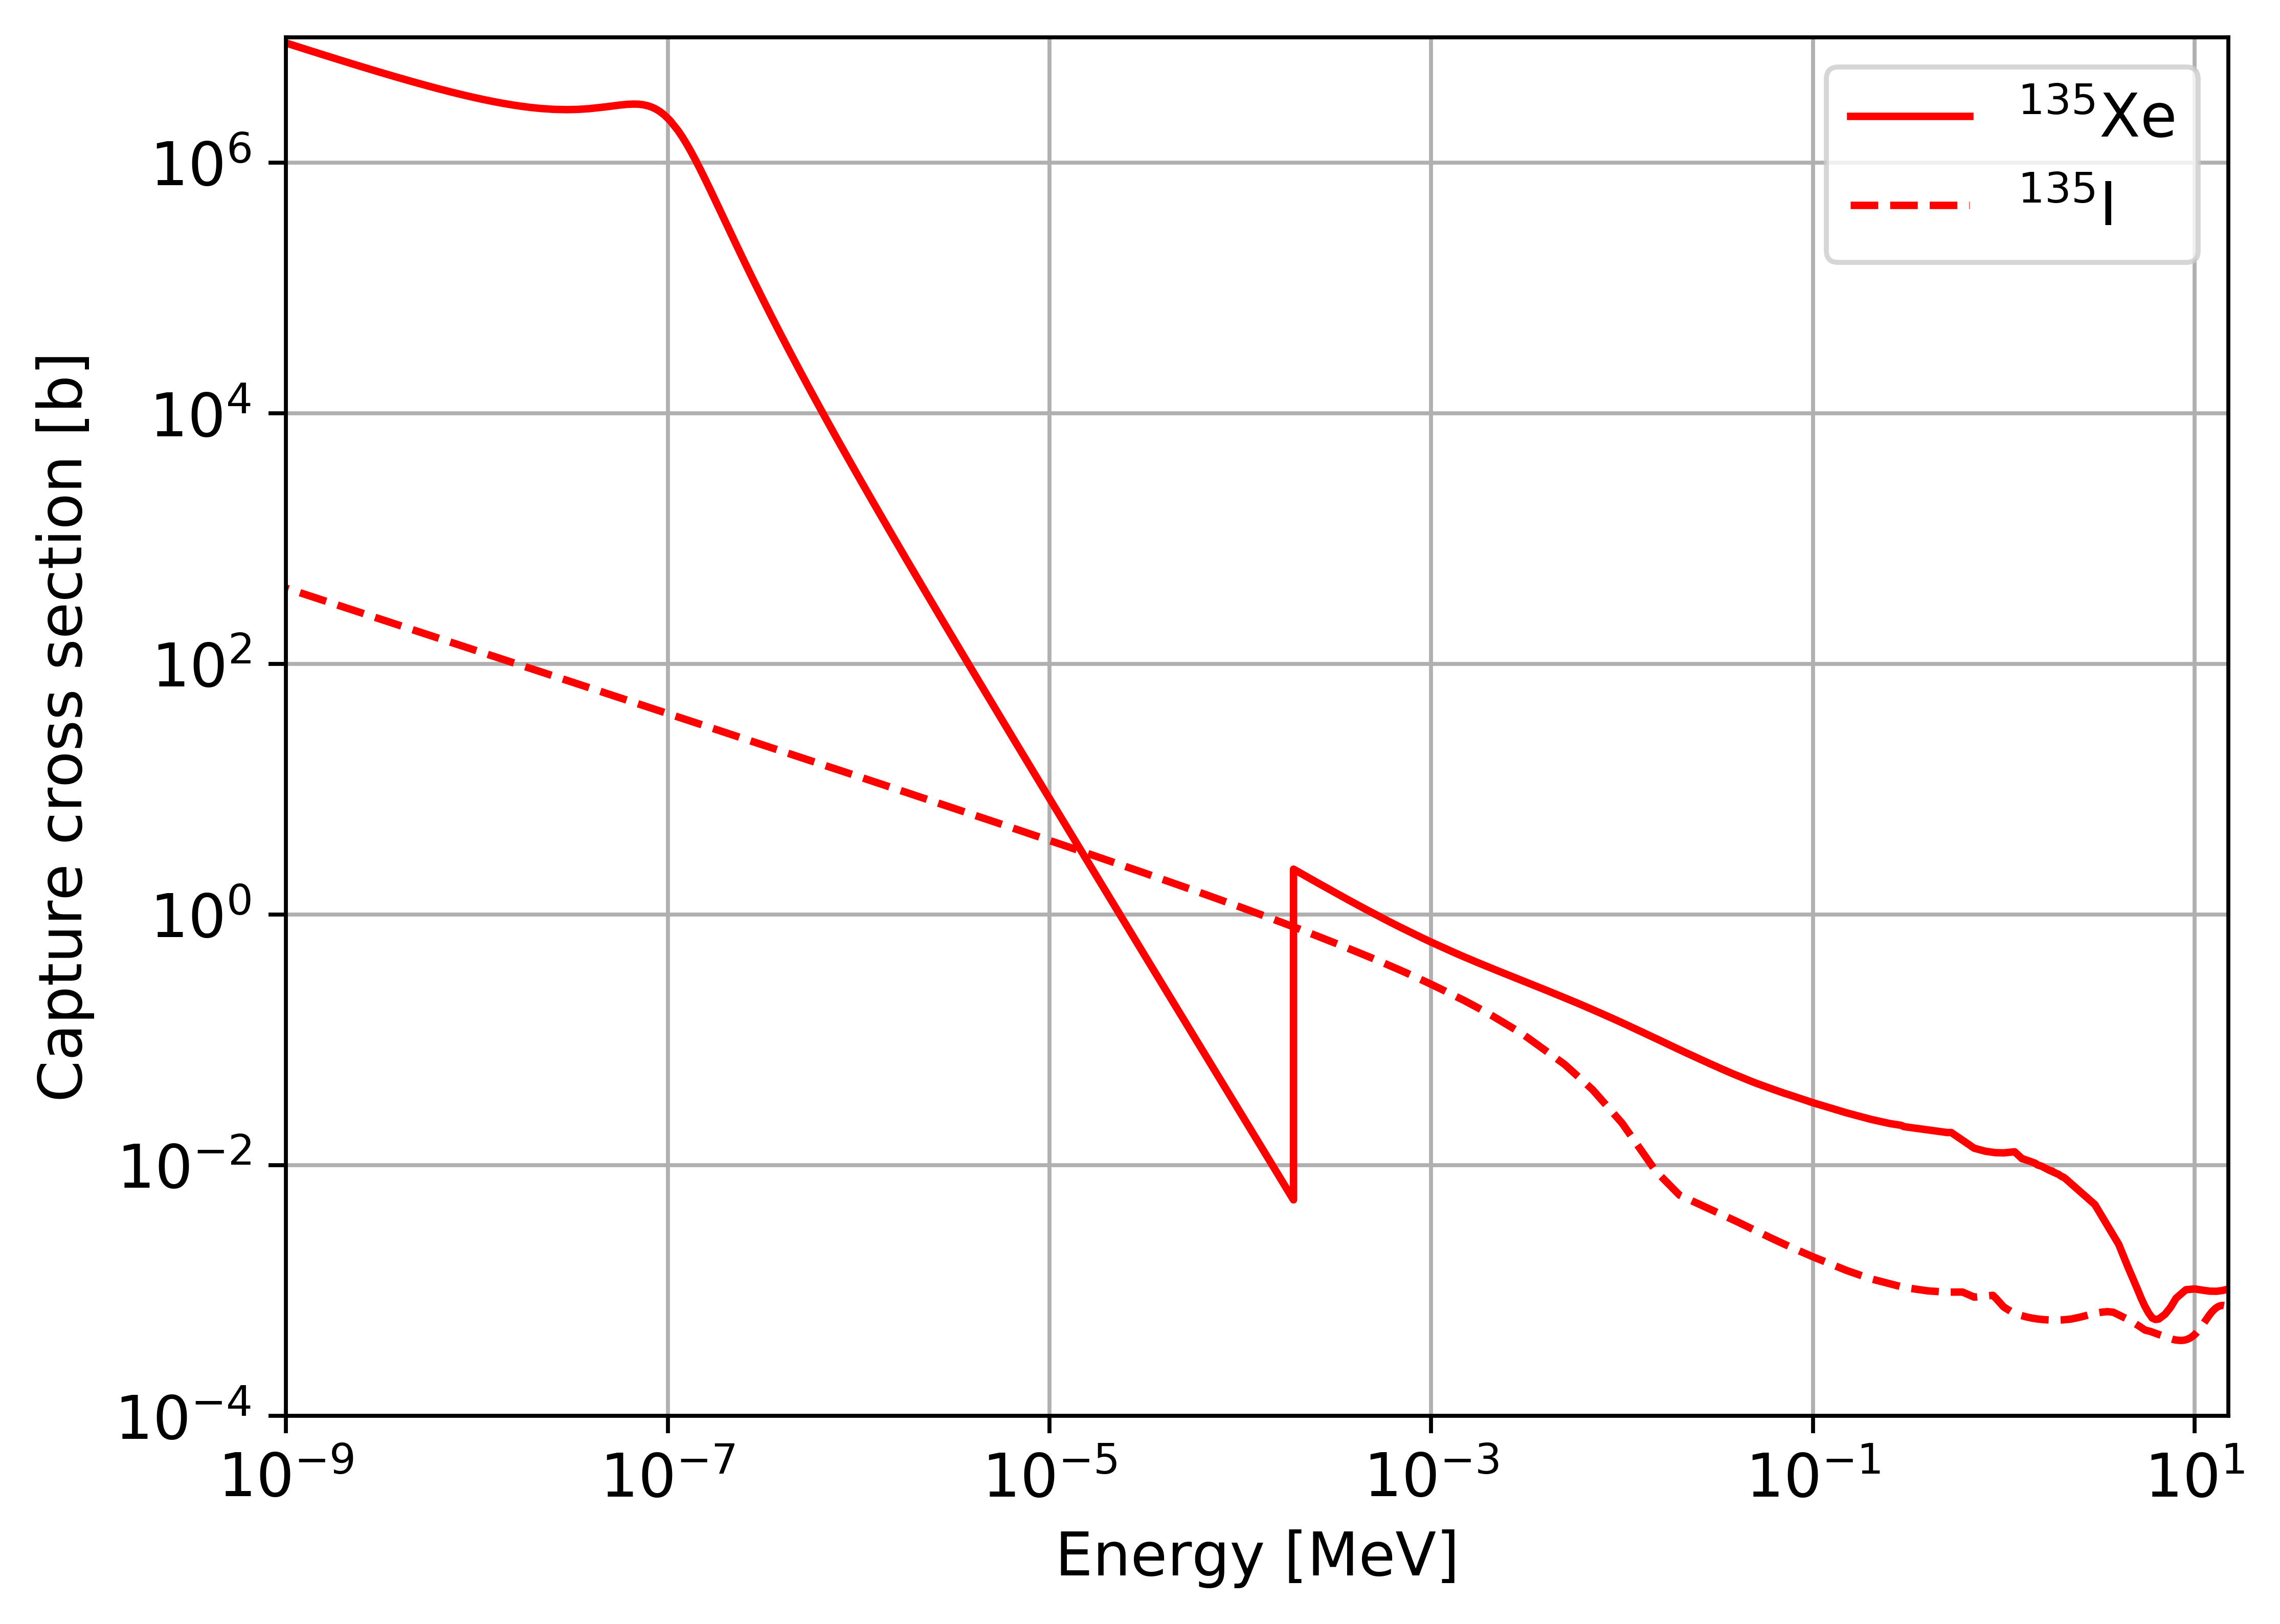
\includegraphics[width=\textwidth]{ch5/i_xe_xs.png}
	\vspace{-8mm}
	\caption{Neutron spectra normalized by lethargy for the \gls{PWR} and 
		\gls{TAP} (upper) and $^{135}$I, $^{135}$Xe caption cross 
		section (lower).}
	\label{fig:tap-pwr-spectrum}
\end{figure}


The \gls{TAP} \gls{MSR} neutron spectrum thermalizes toward the \gls{EOL} due 
to additional moderator rods insertion. Figure~\ref{fig:tap-pwr-spectrum} 
shows that the \gls{TAP} core spectrum at the \gls{EOL} (after 23 years of 
operation, all moderator rods inserted into the core) is thermal and  similar 
to the \gls{PWR} spectrum. However, the $^{135}$I/$^{135}$Xe inventory ratio 
for the \gls{PWR} with fresh fuel is significantly greater than for the 
\gls{TAP} core at the \gls{EOL} despite similar spectra (2.3 and 1.0, 
respectively). The reason for that difference is the different fissile 
content. Results in Section~\ref{sec:long-term} shown that toward the 
\gls{EOL} fissile 
$^{235}$U is being substituted with fissile $^{239}$Pu and $^{241}$Pu. More 
specifically, instead of 6.8 t of $^{235}$U without any plutonium at startup, 
at the \gls{EOL} the fuel salt contains 1.3 t of $^{235}$U, 1 t of 
$^{239}$Pu and 0.5 t of $^{241}$Pu. That is, the fuel salt fissile inventory 
in the \gls{TAP} \gls{MSR} at the \gls{EOL} contains 46 wt\% of $^{235}$U, 36 
wt\% of $^{239}$Pu, and 18 wt\% of $^{241}$Pu.
%Once again, during the \gls{TAP} 
%\gls{MSR} operation a few major changes which impacted $^{135}$I/$^{135}$Xe 
%gain and loss are observed: (1) 
%neutron spectrum is shifted from fast to thermal 
%(Figure~\ref{fig:tap-pwr-spectrum});
%(2) fissile $^{235}$U is substituted with 
%fissile plutonium isotopes (e.g., $^{239}$Pu and $^{241}$Pu). 

Table~\ref{tab:fp-yield-thermal-fission} shows $^{135}$I and $^{135}$Xe yields 
from thermal fission for all fissile isotopes contained in the fuel 
salt. At the \gls{BOL}, the $^{135}$I and $^{135}$Xe in both \gls{TAP} 
reactor and \gls{PWR} are produced from $^{235}$U fission. The rate of 
$^{135}$I isotope production per thermal fission stays approximately the same 
during 23 years of operation because the $^{135}$I yield is very close for all 
considered fissile isotopes. However, the rate of$^{135}$Xe production 
directly from fission for 
fissile plutonium isotopes is significantly greater than for the $^{235}$U 
(e.g., $\approx5$ times greater for $^{239}$Pu and $\approx8$ times greater 
for $^{241}$Pu). Thus, greater $^{135}$Xe production rate with approximately 
the same $^{135}$I production rate leads to smaller $^{135}$I/$^{135}$Xe 
concentration ratio toward \gls{EOL}. Overall, the  $^{135}$I/$^{135}$Xe 
number density ratio increasing from 0.78 to 1.0 during 25 years of the 
\gls{TAP} \gls{MSR} operation, which leads to larger $^{135}$Xe concentration 
peak after shutdown and worsens xenon poisoning effect.
%%%%%%%%%%%%%%%%%%%%%%%%%%%%%%%%%%%%%%%%
\begin{table}[htp!]
	\centering
	\caption{Fission product yields (isotopes per fission) from thermal 
	fission 
	\cite{nichols_handbook_2008}.}
	\begin{tabularx}{0.6\textwidth}{p{0.12\textwidth} R R R}
		\hline
		\textbf{Isotope}  & \textbf{$^{235}$U} &		
		\textbf{$^{239}$Pu} & \textbf{$^{241}$Pu} \\ \hline
		$^{135}$I  & 0.0639 & 0.0633 & 0.0684 \\
		$^{135}$Xe & 0.0022 & 0.0103 & 0.0017 \\
		\hline
	\end{tabularx}
	\label{tab:fp-yield-thermal-fission}
\end{table}
%%%%%%%%%%%%%%%%%%%%%%%%%%%%%%%%%%%%%%%%%%%%%%%%%%%%%%%%%%%%%%%%%%%%%%%%%%%%%%%
%%%%%%%%%%%%%%%%%%%%%%%%%%%%%%%%%%%%%%%%
%\begin{table}[htp!]
%	\centering
%	\caption{Fission product yields (atoms per fission) from fast fission 
%	\cite{nichols_handbook_2008}.}
%	\begin{tabularx}{0.6\textwidth}{p{0.12\textwidth} R R R }
%		\hline
%		\textbf{Isotope}  & \textbf{$^{235}$U} & 
%		\textbf{$^{239}$Pu} & \textbf{$^{241}$Pu} \\ \hline
%		$^{135}$I  & 0.0601 & 0.0624 & 0.0696 \\
%		$^{135}$Xe & 0.0031 & 0.0126 & 0.0030 \\
%		\hline
%	\end{tabularx}
%	\label{tab:fp-yield-fast-fission}
%\end{table}
%%%%%%%%%%%%%%%%%%%%%%%%%%%%%%%%%%%%%%%%%%%%%%%%%%%%%%%%%%%%%%%%%%%%%%%%%%%%%%%



%\section{Prototype design for the xenon removal system}

\section{Safety and operational parameters evolution during load following}
To analyze the impact of the load-following transient on the \gls{TAP} concept 
safety, I calculated safety and operational parameters at various moments 
during postulated earlier worst-case power change transient (0\% power level 
for 11 hours, instantaneous power boost to 100\%, and then 10 hours on 100\% 
power level) using methodology from Section~\ref{sec:safety-param}. The 
combination of fuel and moderator temperature feedback coefficients must 
remain negative during considered short-term transient, and the reactivity 
worth of control rods must be sufficient to shut down the reactor for all 
times during transient. Ideally, the reactor is more controllable if major 
safety and operational parameters remains stable and unaffected by the 
significant power level change.

\subsection{Temperature coefficient of reactivity}
Figure~\ref{fig:lf-tap-tc-evo} shows temperature feedback coefficient 
evolution for the \gls{TAP} reactor during the power change transient. The TC 
increases slightly during the first hour of the transient because a slight 
spectrum hardening due to the $^{135}$Xe concentration peak strengthen the 
Doppler effect in the fuel salt. After turning power back on 100\%, all three 
temperature coefficients of reactivity remains stable because the fuel 
composition remains almost unchanged. Overall, the isothermal temperature 
coefficient, $\alpha_{T,ISO}$ remains negative and strong throughout the 
postulated transient, and fluctuates slightly within stochastic error range 
($\sigma_{\alpha_{T,ISO}}\pm0.043$ $pcm/K$). 
\begin{figure}[htp!] % replace 't' with 'b' to 
	\centering
	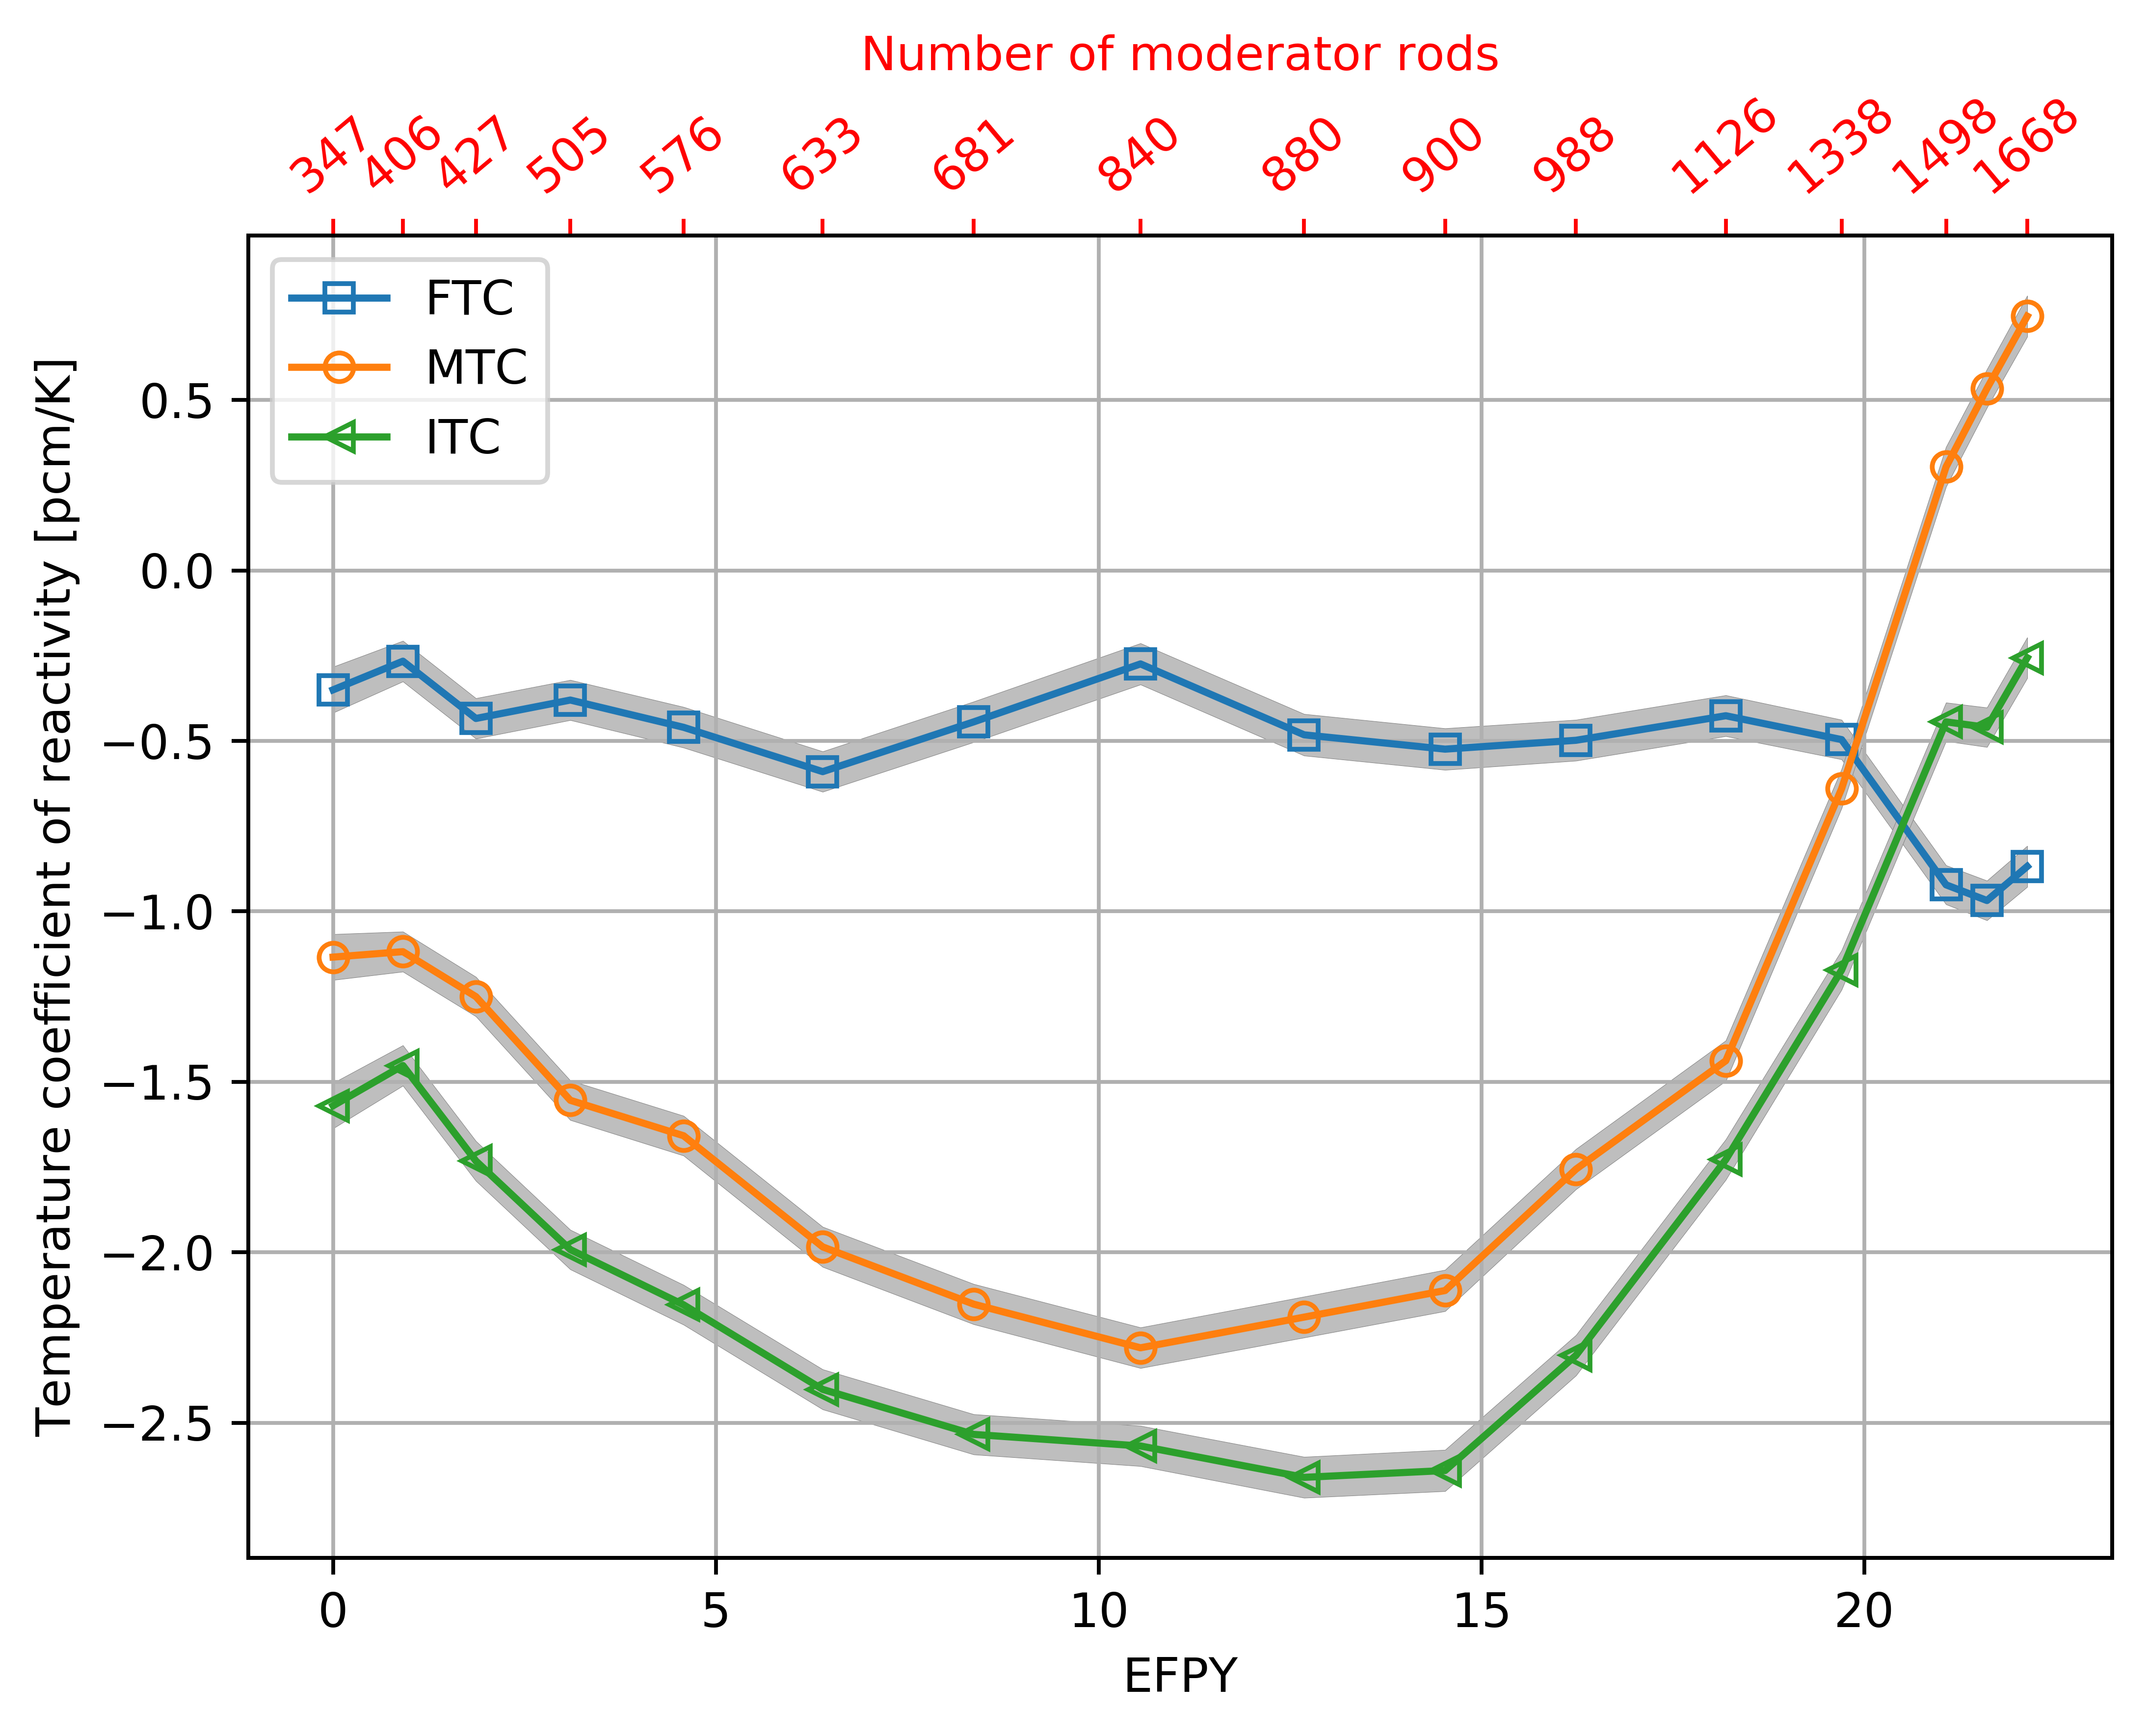
\includegraphics[width=\textwidth]{ch5/saf_par/tc_evo.png}
	\caption{Temperature feedback coefficients evolution during postulated 
		transient for the \gls{TAP} reactor, 10 days before the \gls{EOL} (all 
		moderator rods inserted), the gas removal system operates with 
		efficiency $\epsilon_{Xe}=0.915$. The uncertainty $\pm\sigma$ is 
		shaded.}
		\label{fig:lf-tap-tc-evo}
\end{figure}

\subsection{Void coefficient of reactivity}
Figure~\ref{fig:lf-tap-void-evo} demonstrates void coefficient of reactivity 
evolution during for the \gls{TAP} reactor during the power change transient. 
The coefficient remains almost constant throughout the postulated transient. 
All observed changes of the void coefficient of reactivity are due to 
stochastic nature of the Monte Carlo method ($\sigma_{\alpha_V}\pm4$ $pcm/$\%).
\begin{figure}[htp!] % replace 't' with 'b' to 
	\centering
	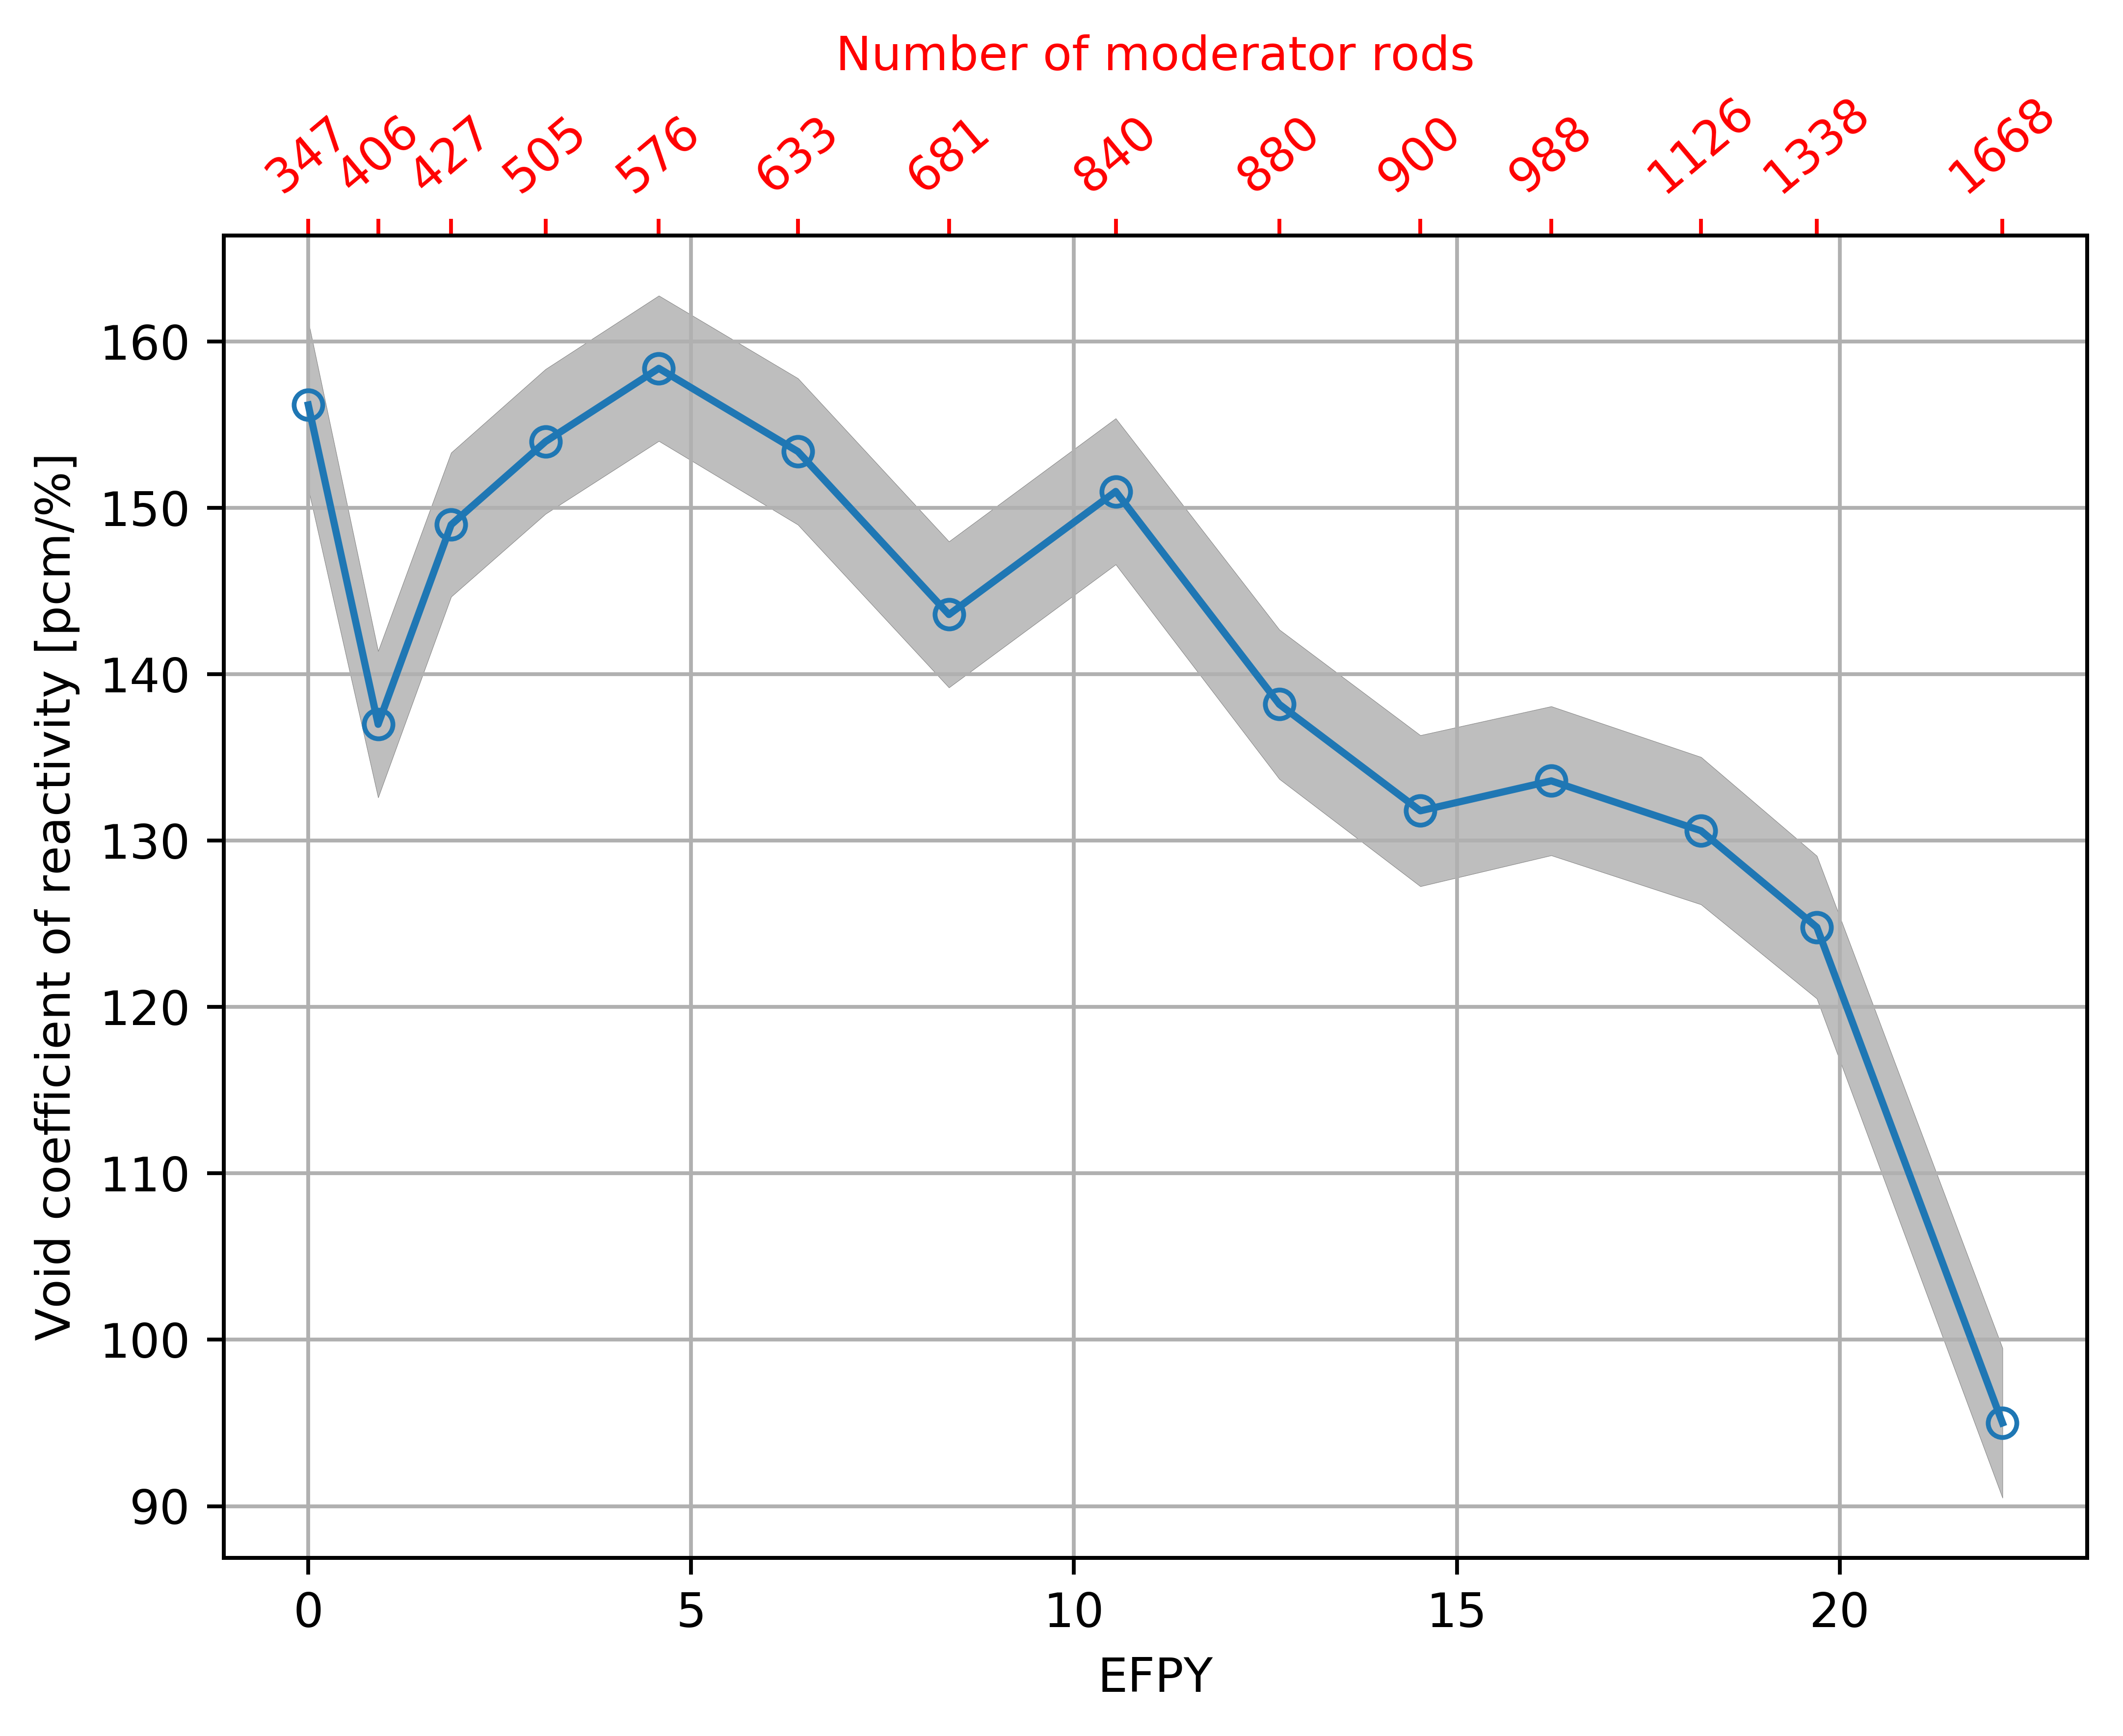
\includegraphics[width=\textwidth]{ch5/saf_par/void_evo.png}
	\caption{Void coefficient of reactivity as a function of time during 
	postulated transient for the \gls{TAP} reactor, 10 days before the 
	\gls{EOL} (all moderator rods inserted), the gas removal system operates 
	with efficiency $\epsilon_{Xe}=0.915$.}
	\label{fig:lf-tap-void-evo}
\end{figure}

\subsection{Reactivity control rod worth}
Figure~\ref{fig:lf-tap-crw-evo} demonstrates control rod worth evolution 
during for the \gls{TAP} reactor during the power change transient. 
The control rod worth remains almost constant and sufficient to shutdown the 
reactor throughout the postulated transient. During first three hours of the 
transient, the control rod worth decreases from $1998.9\pm8.9$ $pcm$ to 
$1988.3\pm8.9$ $pcm$ due to a slight spectrum hardening caused by $^{135}$Xe 
concentration raise. Overall, the changes of control rod worth are 
insignificant and lays within stochastic error range 
($\sigma_{CRW}\pm8.9$ $pcm$).
\begin{figure}[htp!] % replace 't' with 'b' to 
	\centering
	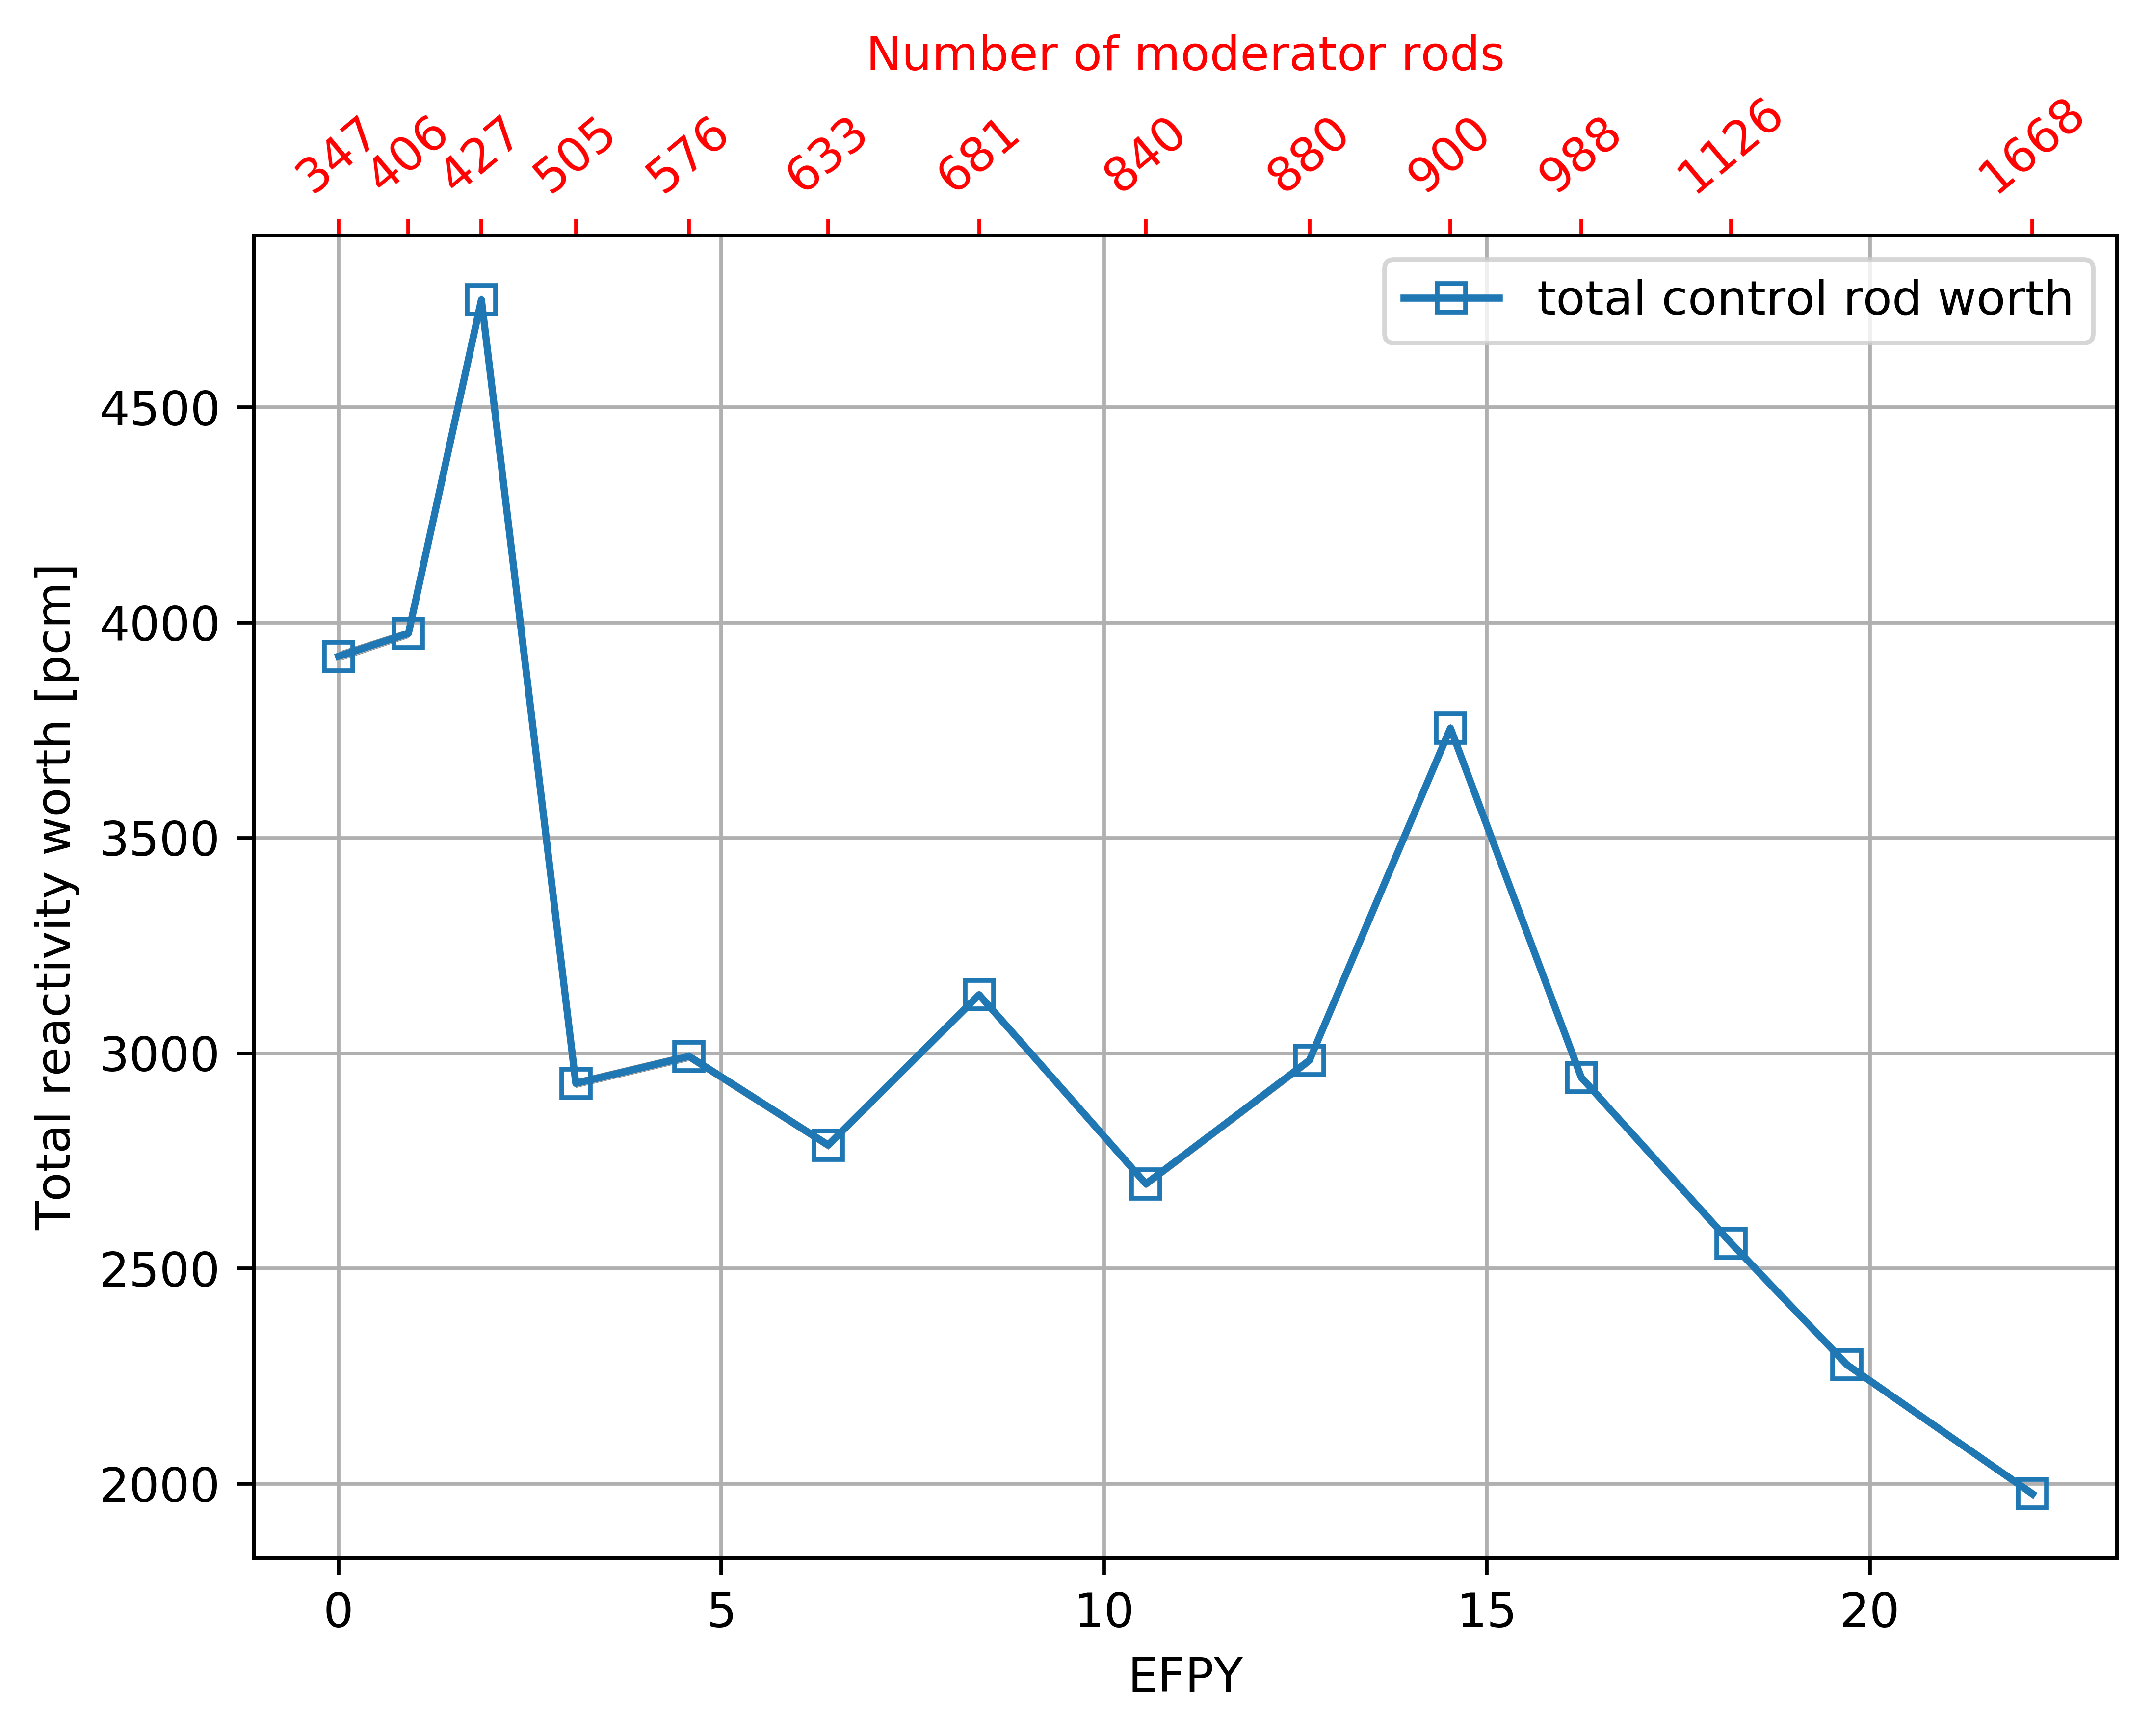
\includegraphics[width=\textwidth]{ch5/saf_par/crw_evo.png}
	\caption{Total control rod worth as a function of time during postulated 
	transient for the \gls{TAP} reactor, 10 days before the \gls{EOL} (all 
	moderator rods inserted), the gas removal system operates with efficiency 
	$\epsilon_{Xe}=0.915$.}
	\label{fig:lf-tap-crw-evo}
\end{figure}


\section{Concluding remarks}
This chapter demonstrated the short-term depletion for the \gls{TAP} reactor
with the core power level variation in the range of [0, 100\%] using SaltProc 
v1.0 and Serpent. I considered two different noble gas removal scenarios: (1) 
inactive gas removal system (e.g., $\epsilon_{Xe}=0$), and (2) fully 
operational gas removal system (e.g., $\epsilon_{Xe}=0.915$, the greatest 
possible efficiency for the system described in 
Section~\ref{sec:tap-online-model}). The current results in literature shown 
that the negative xenon poisoning effect for conventional \glspl{LWR} reaches 
its extremum $\Delta\rho\approx-1500$ $pcm$ in approximately 11 hours after 
shutdown. Such a huge reactivity drop complicates the \glspl{LWR} 
load-following.

This chapter also shows that after the \gls{TAP} reactor shutdown, the 
$^{135}$Xe concentration peaks in about 45 and 165 min at the \gls{BOL} and 
\gls{EOL}, respectively. The xenon peaks sooner for the harder core 
configuration (e.g., at the \gls{BOL}, SVF=0.9) because $^{135}$Xe absorption 
cross section drops dramatically as neutron energy grows above 0.1eV, so, the 
$^{135}$Xe burn out faster in a harder spectrum. Thus, the harder spectrum 
leads to smaller $^{135}$I/$^{135}$Xe concentration ratio and, consequently, 
lower xenon concentration peak. For the inactive gas removal scenario (e.g., 
$^{135}$Xe loss after shutdown due to decay only), xenon concentration at the 
\gls{BOL} remains almost constant ($\Delta N_{^{135}Xe}=+0.33$\%), and no 
effect of xenon poisoning was observed ($\Delta\rho=-10\pm7$ $pcm$). However, 
at the \gls{EOL}, when all moderator rods are in and the neutron spectrum is 
more thermal, I observed more significant effect of poisoning: the $^{135}$Xe 
concentration increased by 4\% with corresponding negative reactivity 
insertion of $-70$ $pcm$. 

For the case with very effective noble gas removal ($\epsilon_{Xe}=0.915$), 
the time when $^{135}$Xe concentration peaks is impossible to predict 
analytically, because after shutdown the gas removal system removes major 
fraction of xenon gas at the end of each depletion step. Moreover, the 
$^{135}$I/$^{135}$Xe ratio is significantly greater (e.g., between 8.66 and 
11.42) than for $\epsilon_{Xe}=0$ case due to very effective xenon removal 
during normal operation on the full power (iodine also being removed but very 
slowly, see Table~\ref{tab:reprocessing_list}). Thus, the $^{135}$I decay 
leads to substantial increase in the $^{135}$Xe concentration right after 
shutdown (up to +200\% at the \gls{EOL}), and corresponding reactivity drop 
($-108\pm5$ $pcm$ at the \gls{EOL}). However, after 1 hour reactivity 
increases quickly because the gas removal system removes most of xenon every 1 
hour, which is predefined SaltProc v1.0 depletion time step. The effect of 
xenon poisoning for the \gls{TAP} reactor with active gas removal system in 
experiments is expected to be even less severe because the system would remove 
noble gases continuously, not discretely as simulated by SaltProc (e.g., xenon 
would be removed with $\epsilon_{Xe}=0.915$ every moment, not once per hour). 
Overall, more realistic results for load-following transients can be obtained 
with better time resolution - depletion time step should be closer to full 
loop time (20 seconds), which can be obtained with enormous computation burden.

Finally, this chapter demonstrated that the \gls{TAP} reactor maintains major 
safety margins during postulated transients. The temperature feedback 
coefficients, void coefficient of reactivity, and control rod worth all remain 
within stochastic uncertainty throughout the transient. Small elevation in 
total temperature coefficient and void coefficient of reactivity during the 
first hour after shutdown is due to the $^{135}$Xe concentration raise and 
corresponding short-term neutron spectrum hardening. In conclusion, the 
\gls{TAP} \gls{MSR} even with switched off gas removal system is capable to 
reduce power from 100\% to 0\% and then restart even when the $^{135}$Xe 
concentration culminate without compromising critical safety margins. 
Comprehensive material study must be done to prove that structural materials 
could withstand such a dramatic core power fluctuations.





